%%
%% Dibbler - a portable DHCPv6
%%
%% authors: Tomasz Mrugalski <thomson@klub.com.pl>
%%          Marek Senderski <msend@o2.pl>
%%
%% released under GNU GPL v2 only licence
%%
%% $Id: dibbler-user.tex,v 1.20 2008-08-29 00:07:38 thomson Exp $
%%

\documentclass[11pt]{article}
\usepackage[latin2]{inputenc}
\usepackage[dvips]{graphicx}
\usepackage{float}
\usepackage{makeidx}
\usepackage{fancyhdr}
\usepackage{indentfirst}
\usepackage{tabularx}
\usepackage{longtable}
\usepackage{url}
\usepackage[usenames]{color}
\usepackage[colorlinks=true,citecolor=darkblue,linkcolor=darkblue,urlcolor=darkred]{hyperref}

%\setlength{\topmargin}{-1.0cm}
\usepackage[twoside=true,
	    left={2cm},
	    right={2cm},
	    top={2cm},
	    bottom={2cm},
	    footskip={1cm},
	    headheight={1cm},
%%            twosideshift={0.5cm},
	    headsep={0.5cm}]{geometry}

%%%%%% \dzis macro by Lupan %%%%%%
\newcommand{\dzis}{
\the\year-%
\ifnum\month<10{}0\fi
\the\month-%
\ifnum\day<10{}0\fi
\the\day
}

\author{Tomasz Mrugalski\\ \small{\href{mailto:thomson(at)klub.com.pl}{thomson(at)klub.com.pl}}}
\date{\dzis}
\title{Dibbler -- a portable DHCPv6\\User's guide}

\definecolor{myBgColor}{rgb}{1.0,1.0,1.0}
\definecolor{darkred}{rgb}{0.7,0.2, 0.4} %% URL (external links)
\definecolor{darkblue}{rgb}{0.0,0.0,0.7} %% internal links, toc
\definecolor{myBgTableColor}{rgb}{0.9, 0.9, 0.9}
\pagecolor{myBgColor}

\pagestyle{fancy}
\fancyhf{}
\fancyhead[L]{\small\bfseries Dibbler -- a portable DHCPv6}
\fancyhead[C]{\small\bfseries User's Guide}
\fancyhead[R]{\small\bfseries\thepage}
%%\fancyhead[C]{\small\bfseries\leftmark}
\renewcommand{\headrulewidth}{0.5pt}
\renewcommand{\footrulewidth}{0pt}
\addtolength{\headheight}{0.5pt}
\fancypagestyle{plain}{%
\fancyhead{} %
\renewcommand{\headrulewidth}{0pt} %
}

%%\newenvironment{Cfg}{ \Verbatim }{ \endVerbatim }

\makeindex

\newcommand{\Q}{ \vspace{0.5cm} \textbf{Q:} }
\newcommand{\A}{ \vspace{0.25cm} \textbf{A:} }
\newcommand{\Note}{ \textbf{Note:} }

\newcommand{\msg}[1]{\emph{#1}}
\newcommand{\opt}[1]{\emph{#1}}
\newcommand{\IA}{ \textbf{\emph{IA}} }
\newcommand{\duid} { DUID }
\newcommand{\code}[1]{\textbf{#1}}
\newcommand{\subsubsubsection}[1]{\subsubsection{#1}}
\newcommand{\CfgBegin}{\begin{lstlisting}}
\newcommand{\CfgEnd}{\end{lstlisting}}

%% this does not work... yet
\newenvironment{Cfg}{\begin{lstlisting}}{\end{lstlisting}}

%% for Verbatim environment
%%\RecustomVerbatimEnvironment{Verbatim}{Verbatim}{frame=single,framesep=3mm}

%%\renewcommand{\FancyVerbFormatLine}[1]{\colorbox{red}{#1}}
\usepackage{listings}
\lstset{basicstyle=\ttfamily, columns=flexible, backgroundcolor=\color{myBgTableColor},frame=lines}
%or columns=fullflexible

%% include auto-generated version number
\input{version.tex}

%% message names should be printed this way: \msg{SOLICIT}
%% options should be printed this way:       \opt{Option Request}

\begin{document}

\vspace{-4cm}
\maketitle
\vspace{-1cm}

\begin{center}
\version
\end{center}

\newpage
\tableofcontents

\newpage

%% INTRO, OVERVIEW
%%
%% $Id: dibbler-user-intro.tex,v 1.5 2005-01-23 23:16:56 thomson Exp $
%%
%% $Log: not supported by cvs2svn $
%% Revision 1.4  2004/10/25 20:45:54  thomson
%% Option support, parsers rewritten. ClntIfaceMgr now handles options.
%%
%% Revision 1.3  2004/06/19 19:51:14  thomson
%% Various fixes.
%%
%% Revision 1.2  2004/06/19 10:24:59  thomson
%% Hyperlinks in PDF, building process modified
%%
%%

\section{Intro}
First of all, as an author I would like to thank you for your interest
in this DHCPv6 implementation. If this documentation doesn't answer
your question or you have any suggestions, feel free to contact
me. See \emph{Contact} section for details. Also be sure to check out
Dibbler website located at \url{http://klub.com.pl/dhcpv6/}.

%%\href{http://klub.com.pl/dhcpv6/}{Dibbler's website}.

\section{Overview}

Dibbler is a portable DHCPv6 solution. It features server, client and
relay. Currently there are ports available for Windows XP and 2003
and Linux systems. Besides basic functionality specified in RFC3315,
it also offers serveral enhancements, e.g. DNS servers and doman names
configuration.

Dibbler is an open source software, distributed under GNU GPL
licence. It means that it is freely available, free of charge and can
be used by anyone (including commercial users). Sources are also
available, so anyone skilled enough can fix bugs or add new features.

As for now, Dibbler offers these features:
\begin{itemize}
\item Basic server discovery and address assignment (SOLICIT,
  ADVERTISE, REQUEST and REPLY messages) -- simplest case possible:
  client discovers server, then asks for an address, which is granted
  by a~server.
\item Best server discovery -- when client receives more than one
  ADVERTISE messages from different servers, it chooses the best one
  and remembers remaining ones as a backup.
\item Many servers support -- client is capable of discovering and
  dealing with multiple servers. For example, client would like to
  have 5 addresses configured. Prefered server can only grant 3, so
  client send request for remaining 2 addresses to one of the
  remaining servers.
\item Relay support -- Dibbler server supports indirect
  communication with clients via relays. Relay implementation is also
  available. Clients can talk to the server directly or via relays.
\item Unicast communication -- if specific conditions are met, client
  could send messages directly to a server's unicast address, so
  additional servers does not need to process those messages. It also
  improves effciency, as all nodes present in LAN segment receive
  multicast packets.\footnote{Nodes, which do not belong to specific
    multicast group, drop those packets silently. However, determining
    if host belongs or not to a group must be performed on each node.}
\item Address renewal (RENEW,REBIND and REPLY messages) -- client renews
  addresses at certain time intervals, if server specified so.
\item Duplicate address detection (DECLINE and REPLY messages) -- client
  can detect and properly handle faulty situation, when server grants
  address which is illegaly used by some other host. It will inform
  server of such circumstances, and request for another
  address. Server will mark this address as used by unknown host, and
  will assign another address to a client.
\item Power failure/crash support (CONFIRM and REPLY messages) -- after
  client recovers from crash or power failure, it still can have
  assigned valid addresses. In such circumstances, client uses CONFIRM
  message, to config if those addresses are still valid%
  \footnote{As for 0.3.1 version, this functionality works on server side only,
  client side support will be available in 0.4.0.}.
\item IA Option -- this option is used to carry addresses. Both server
  and client support multiple IAs in one message. Additional feature
  is client capability to ask for a specific address.
\item Rapid Commit Option (SOLICIT and REPLY messages) -- if both
  client and server are configured to use rapid commit, address
  assignment procedure can be shortened to 2 messages. Major
  advantage is lesser network usage and quicker client startup time.
\end{itemize}

Except RFC3315-specified behavior, Dibbler also support several enhancements:

\begin{itemize}
\item DNS Servers Option -- client can ask for information about DNS
  servers.
\item Domain Name Option -- client can ask for information about
  domain name it is connected in.
\item Time Zone Option -- client can ask for information about 
time zone it is currently in.
\item NTP Servers Option -- client can ask for Network Time Protocol
  Servers to synchronize its clock.
\item SIP Servers Option -- SIP servers IPv6 address information can
  be passed to clients.
\item SIP domain name - SIP domain name can be passed to clients.
\item NIS, NIS+ server Option -- Both NIS and NIS+ server adresses
  can be passed to clients.
\item NIS, NIS+ domain name Option -- NIS or NIS+ domain names can be
  passed to clients.
\item Option renewal mechanism (Lifetime Option) -- options obtained
  from server can be updated periodically.
\end{itemize}

And now some implementation specific details:
\begin{itemize}
\item On Server, client and relay, after each modification data is
  dumped in XML format, so it can be easily processed in an automated
  manner. Simple example of this advantage is a script, which can generate
  reports about server usage (assigned addresses, clients configured
  and so on);
\item Dibbler is fully portable. Core logic is system independent and
  coded in C++ language. There is about dozen low-level functions,
  which are system speficic. They're used for adding addresses,
  retriving information about interfaces, setting DNS servers and so
  on. Porting Dibbler to other systems (and even other architectures)
  would require implementic only those serveral system-specific
  functions.
\end{itemize}

See RELEASE-NOTES for details about version-specific upgrades, fixes
and features.

%% INSTALLATION and USAGE
%%
%% Dibbler - a portable DHCPv6
%%
%% authors: Tomasz Mrugalski <thomson@klub.com.pl>
%%
%%
%% released under GNU GPL v2 licence
%%

\newpage
\section{Installation and usage}
\label{install}
Client, server and relay are installed in the same way. Installation
method is different in Windows and Linux systems, so each system
installation is described separately. To simplify installation, it
assumes that binary versions are used\footnote{Compilation is not
required, usually binary version can be used. Compilation should be
performed by advanced users only, see Section \ref{compile} for
details.}.

\subsection{Linux installation}
Starting with 0.4.0, Dibbler consists of 3 different elements: client,
server and relay. During writing this documentation, Dibbler is already
part of many Linux distributions. In particular:
\begin{description}
 \item[\href{http://debian.org}{Debian
 GNU/Linux}, \href{http://ubuntu.com}{Ubuntu}] and derived -- use
 standard tools (apt-get, aptitude and similar) to install
 dibbler-client, dibbler-server, dibbler-relay or dibbler-doc packages.
\item[\href{http://opensuse.org}{OpenSUSE}] -- use standard
 installation mechanism.
\item[\href{http://www.pld-linux.org}{PLD GNU/Linux}]
 -- use standard PLD's poldek tool to install dibbler
 package.  \item[\href{http://www.gentoo.org}{Gentoo Linux}] -- use
 emerge to install dibbler (e.g. emerge dibbler).
\item[\href{http://openwrt.org}{OpenWRT}] -- there are package
 definitions for OpenWRT. At time of this writing, they were very
 outdated (using 0.5.0 version).
\end{description}

If you are using other Linux distribution, check out if it already
provides Dibbler packages. You may use them or compile the sources on
your own. See Section \ref{compile} for details regarding compilation
process. Dibbler used to provide native DEB and RPM packages, but due
to limited resources, author is not continuing this activity. If you
are a Dibbler package maintainer and want your package to be put on
dibbler website, please send such request on mailing list (see
Section \ref{mailing-list}).

To install Dibbler on Debian or other system that provides apt-get
package management system, run \verb+apt-get install package+
command. For example, to install server and client, issue the
following command:

\begin{lstlisting}
apt-get install dibbler-server dibbler-client
\end{lstlisting}

To install Dibbler in Gentoo systems, just type:
\begin{lstlisting}
emerge dibbler
\end{lstlisting}

\subsection{Windows installation}
Dibbler supports Windows XP and 2003 since the 0.2.1-RC1 release.
Support for Vista was added somewhere around 0.7.x. Support for
Windows 7 was added in 0.8.0RC1. In version 0.4.1 exprimental support
for Windows NT4 and 2000 was added. The easiest way of Windows
installation is to download clickable Windows installer. It can be
downloaded from \url{http://klub.com.pl/dhcpv6/}. After downloading,
click on it and follow on screen instructions. Dibbler will be
installed and all required links will be placed in the Start
menu. Note that there are two Windows versions (ports): one for modern
systems (XP/2003/Vista and Win7) and one for archaic ones
(NT4/2000). Make sure to use proper port. If you haven't set up IPv6
support, see following sections for details.

Operation on Windows 8 was never tested, so support is not confirmed.

\subsection{Mac OS X installation}
As of 0.8.0 release, ready to use dmg packages are not provided,
therefore dibbler has to be compiled. Please follow section
\ref{compile} for generic Dibbler compilation that applies to Mac OS
X.

Currently support for Mac OS X is usable, but there is still one
notable limitation. Client is not able to configure DNS servers or
domain name informations.

\subsection{FreeBSD, NetBSD, OpenBSD}
As of 0.8.1RC1 release, support for FreeBSD, NetBSD and OpenBSD has
been added. There are no prebuilt binary packages available. Please
follow Section \ref{compile} for generic Dibbler compilation that applies to
all 3 mentioned OSes.


\subsection{Basic usage}
Depending what functionality do you want to use (server,client or relay),
you should edit configuration file (\verb+client.conf+ for client, \verb+server.conf+
for server and \verb+relay.conf+ for relay). All configuration files should
be placed in the \verb+/etc/dibbler+ directory. Also make sure that
\verb+/var/lib/dibbler+ directory is present and is writeable. After
editing configuration files, issue one of the following commands:

\begin{lstlisting}
dibbler-server start
dibbler-client start
dibbler-relay start
\end{lstlisting}

\verb+start+ parameter requires little explanation. It
instructs Dibbler to run in daemon mode -- detach from console and run
in the background. During configuration files fine-tuning, it is ofter better
to watch Dibbler's bahavior instantly. In this case, use \verb+run+
instead of \verb+start+ parameter. Dibbler will present its messages on
your console instead of log files. To finish it, press ctrl-c.

To stop server, client or relay running in daemon mode, type:
\begin{lstlisting}
dibbler-server stop
dibbler-client stop
dibbler-relay stop
\end{lstlisting}

To see, if client, server or relay are running, type:

\begin{lstlisting}
dibbler-server status
dibbler-client status
dibbler-relay status
\end{lstlisting}

To see full list of available commands, type \verb+dibbler-server+,
\verb+dibbler-client+ or \verb+dibbler-relay+ without any parameters.

If your OS uses different layout of directories, you may want to
modify Misc/Portable.h before starting compilation process.

\newpage
\section{Compilation}
\label{compile}
Dibbler is distributed in 2 versions: binary and source code. If there
is binary version provided for your system,  it is usually better
choice.  Compilation usually is performed by more experienced users.
In average case it does not offer significant advantages over binary version.
You probably want to just install and use Dibbler. If that is your case, read section
named \ref{install}. However, if you are skilled enough, you might
want to tune several Dibbler aspects during compilation. See \emph{
Dibbler Developer's Guide} for information about various compilation
parameters.

\subsection{Linux/Mac OS X/FreeBSD/NetBSD/OpenBSD Compilation}
The following descriptions applies to Linux, Mac OS X, FreeBSD, NetBSD
and OpenBSD. Other POSIX systems may work, but were never tested by
author. If you would like to install Dibbler from sources, you will need all
required dependencies. In particular, you need a typical C++
environment: a C and C++ compilers (most probably gcc and g++), make,
and several other smaller tools.

To install Dibbler package from sources, go to project homepage and
download latest tar.gz source archive. Extract it using available tool
for that purpose (in most cases that would be tool called tar and
gzip).

After sources are extracted, they must be configured to match specific
operating system. To complete this step, a configure script must be
called:
\begin{lstlisting}
./configure
\end{lstlisting}

Configure script accepts many parameters, so if like to tweak
something, here is your chance. You may run \verb+./configure --help+
to see list of available parameters. For example, to set up sources to
compile in debug mode (useful if you want to debug them or provide
better bugreport), you can do this:

\begin{lstlisting}
./configure --enable-debug
\end{lstlisting}

Once configure completes its operation, it prints out details of its
configuration and source are ready for compilation. To build all
components, just type make. If you want to make specific component
only, you may use it as parameter to make, e.g. 
\verb+make server+. After successful compilation type \verb+make install+ to
install compiled code in your system.

For example, to build server and relay, type:

\begin{lstlisting}
tar zxvf dibbler-0.8.1RC1-src.tar.gz
./configure
make server relay
make install
mkdir -p /var/lib/dibbler
\end{lstlisting}

Configure script was added in 0.8.1RC1. Earlier versions do not not
need that step.

Dibbler was compiled using gcc 2.95, 3.0, 3.2, 3.3, 3.4, 4.0, 4.1,
4.2, 4.3, 4.4 and 4.5 versions. Note that many older compilers are is
now considered obsolete and ware not tested for some time. Lexer files
(grammar defined config file) were generated using flex 2.5.33. Parser
file were created using bison++ 1.21.9. Flex and bison++ tools are not
required to compile Dibbler. Generated files are placed in GIT and in
tar.gz archives. Dibbler requires also make. Autoconf and automake
tools (autotools) were used for regeneration of the Makefiles and
configure script.
 
\subsection{Modern Windows (XP...Win7) compilation}
Download dibbler-\version-src.tar.gz and extract it. In
\verb+Port-win32+ there are several project files (for server, client
and relay) for MS Visual Studio 2008. According to authors knowledge,
it is possible to compile dibbler using free MS Visutal C++ Express
2008 edition. Previous dibbler releases were compiled using MS Visual
Studio .NET (sometimes called 2002) and 2003. Those versions are not
supported anymore. It might work with newest dibber version, but there
are no guarantee. Open \verb+dibbler-win32.vs2008.sln+ solution file
click Build command. That should start compilation. After a while,
binary exe files will be stored in the \verb+Debug/+ or
\verb+Release/+ directories.

\subsection{Legacy Windows (NT/2000) compilation}
Windows NT4/2000 port is considered experimental, but there are reports
that it works just fine. To compile it, you should download dev-cpp
(\url{http://www.bloodshed.net/dev/devcpp.html}), a free IDE for
Windows utilising minGW port of the gcc for Windows. Run dev-cpp,
click ,,open project...'', and open one of the \verb+*.dev+ files located
in the Port-winnt2k directory, then click compile. You also should
take a look at \verb+Port-winnt2k/INFO+ file for details.


\subsection{IPv6 support}
Some systems does not have IPv6 enabled by default. In that is the case,
you can skip following subsections safely. If you are not sure, here is
an easy way to check it. To verify if you have IPv6 support, execute
following command: \verb+ping6 ::1+ (Linux) or \verb+ping ::1+
(Windows). If you get replies, you have IPv6 already installed.

\subsubsection{Setting up IPv6 in Linux}
Almost all modern Linux distributions have IPv6 enabled by default, so there
is very good chance that nothing has to be done. However, if that is
not the case, IPv6 can be enabled in Linux systems in two ways:
compiled directly into kernel or as a module. If you don't have IPv6
enabled, try to load IPv6 module: \verb+modprobe ipv6+ (command
executed as root) and try \verb+ping6 ::1+. If that fails, you have to
recompile kernel to support IPv6. There are numerous descriptions how
to recompile kernel available on the web, just type "kernel
compilation howto" in \href{http://www.google.com}{Google}.

\subsubsection{Setting up IPv6 in Windows Vista and Win7}
Both systems have IPv6 enabled by default. Also note that Win7 also
has DHCPv6 client built-in, so you may use it as well.

\subsubsection{Setting up IPv6 in Windows XP and 2003}
If you have already working IPv6 support, you can safely skip this section.
The easiest way to enable IPv6 support is to right click on the
\verb+My network place+ on the desktop, select \verb+Properties+, then locate
your network interface, right click it and select \verb+Properties+. Then
click \verb+Install...+, choose protocol and then IPv6 (its naming is
somewhat diffrent depending on what Service Pack you have installed).
In XP, there's much quicker way to install IPv6. Simply run command
\verb+ipv6 install+ (i.e. hit Start..., choose run... and then type
\verb+ipv6 install+). Also make sure that you have built-in firewall
disabled. See \emph{Frequently Asked Question} section for details.

\subsubsection{Setting up IPv6 in Windows 2000}
If you have already working IPv6 support, you can safely skip this
section. The following description was provided by Sob (
(\href{mailto:sob(at)hisoftware.cz}{sob(at)hisoftware.cz}). Thanks. This
description assumes that ServicePack 4 is already installed.

\begin{enumerate}
  \item Download the file tpipv6-001205.exe from:
    \url{http://msdn.microsoft.com/downloads/sdks/platform/tpipv6.asp}
    and save it to a local folder (for example, \verb+C:\IPv6TP+).
  \item From the local folder (\verb+C:\IPv6TP+), run
    \verb+Tpipv6-001205.exe+ and extract the files to the same
    location.
  \item From the local folder (\verb+C:\IPv6TP+), run
    \verb+Setup.exe -x+ and extract the files to a subfolder of the
    current folder (for example, \verb+C:\IPv6TP\files+).
  \item From the folder containing the extracted files
    (\verb+C:\IPv6TP\files+), open the file \verb+Hotfix.inf+ in a
    text editor.
  \item In the [Version] section of the Hotfix.inf file, change the
    line NTServicePackVersion=256 to NTServicePackVersion=1024, and
    then save changes. \footnote{This defines Service Pack
      requirement.  NTServicePackVersion is a ServicePack version
      multiplied by 256. If there would be SP5 available, this value
      should have been changed to the 1280.}
  \item From the folder containing the extracted files
    (\verb+C:\IPv6TP\files+), run \verb+Hotfix.exe+.
  \item Restart the computer when prompted.
  \item After the computer is restarted, from the Windows 2000
    desktop, click Start, point to Settings, and then click Network
    and Dial-up Connections. As an alternative, you can right-click My
    Network Places, and then click Properties.
  \item Right-click the Ethernet-based network interface to which you
    want to add the IPv6 protocol, and then click
    Properties. Typically, this network interface is named Local Area
    Connection.
  \item Click Install.
  \item In the Select Network Component Type dialog box, click
    Protocol, and then click Add.
  \item In the Select Network Protocol dialog box, click Microsoft
    IPv6 Protocol and then click OK.
  \item Click Close to close the Local Area Connection Properties
    dialog box.
\end{enumerate}

\subsubsection{Setting up IPv6 in Windows NT4}
If you have already working IPv6 support, you can safely skip this
section.  The following description was provided by The following
description was provided by Sob
(\href{mailto:sob(at)hisoftware.cz}{sob(at)hisoftware.cz}). Thanks.

\begin{enumerate}
  \item Download the file msripv6-bin-1-4.exe from:
    \url{http://research.microsoft.com/msripv6/msripv6.htm}{Microsoft}
    and save it to a local folder (for example, \verb+C:\IPv6Kit+).
  \item From the local folder (\verb+C:\IPv6Kit+), run
    \verb+msripv6-bin-1-4.exe+ and extract the files to the same
    location.
  \item Start the Control Panel's "Network" applet (an alternative way to do this is
    to right-click on "Network Neighborhood" and select "Properties") and select
    the "Protocols" tab.
  \item Click the "Add..." button and then "Have Disk...". When it asks you for
    a disk, give it the full pathname to where you downloaded the binary
    distribution kit (\verb+C:\IPv6Kit+).
  \item IPv6 is now installed.
\end{enumerate}


%% FEATURES
\section{Features HOWTO}
This section contains information about setting up various Dibbler
features. Since this section was added recently, it is not yet
comprehensive. That is expected to change.

\subsection{Stateless vs stateful and IA, TA options}
\label{features-stateless-stateful}
This section explains the difference between stateless and stateful
configurations. IA and TA options usage is also described.

Usually, normal stateful configuration based on non-temporary
addresses should be used. If you don't know, what temporary addresses
are, you don't need them.

There are two kinds of configurations in DHCPv6 (\cite{rfc3315}, \cite{rfc3736}):
\begin{description}
  \item[stateful] -- it assumes that addresses (and possibly other parameters)
    are assigned to a client. To perform this kind of configuration,
    four messages are exchanged: \msg{SOLICIT}, \msg{ADVERTISE},
    \msg{REQUEST} and \msg{REPLY}.
  \item[stateless] -- when only parameters are configured (without
    assigning addresses to a client). During execution of this type of
    configuration, only two messages are exchanged: \msg{INF-REQUEST}
    and \msg{REPLY}.
\end{description}

During normal operation, client works in a stateful mode. If not
instructed otherwise, it will request one or more normal (i.e. non-temporary)
address. It will use \opt{IA} option (Identity Association for
Non-temporary Addresses, see \cite{rfc3315} for details) to request
and retrieve addresses. Since this is a default behavior, it does not
have to be mentioned in the client configuration
file. Nevertheless, it can be provided:

\begin{lstlisting}
# client.conf
iface eth0 {
  ia
  option dns-server
}
\end{lstlisting}

In a specific circustances, client might be interested in obtaining
only temporary addresses. Although this is still a stateful mode, its
configuration is sligtly different. There is a special option called \opt{TA}
(Identity Association for Temporary Addresses, see \cite{rfc3315} for
details). This option will be used to request and receive temporary
addresses from the client. To force client to request temporary
addresses instead of permanent ones, \verb+ta+ keyword must be used in
client.conf file. If this option is defined, only temporary address
will be requested. Keep in mind that temporary addresses are not
renewed.

\begin{lstlisting}
# client.conf
iface eth0 {
  ta
  option dns-server
}
\end{lstlisting}

It is also possible to instruct client to work in a stateless mode. It
will not ask for any type of addresses, but will ask for specific
non-adress related configuration parameters, e.g. DNS Servers
information. This can be achieved by using \verb+stateless+
keyword. Since this is a global parameter, it is not defined on any
interface, but as a global option.

\begin{lstlisting}
# client.conf
stateless
iface eth0
{
  option dns-server
}
\end{lstlisting}

Some of the cases mentioned above can be used together. However,
several combinations are illegal. Here is a complete list:
\begin{description}
\item[none] -- When no option is specified, client will assume one IA
	   with one address should be requested. Client will send
	   \verb+ia+ option (stateful autoconfiguration).
\item[ia] -- Client will send \verb+ia+ option (stateful
  autoconfiguration).
\item[ia,ta] -- When both options are specified, client will request
  for both - Non-temporary as well as Temporary addresses (stateful
  autoconfiguration).
\item[stateless] -- Client will request additional configration
  parameters only and will not ask for addresses (stateless
  autoconfiguration).
\item[stateless,ia] -- This combination is not allowed.
\item[stateless,ta] -- This combination is not allowed.
\item[stateless,ia,ta] -- This combination is not allowed.
\end{description}

\subsection{DNS Update}
\label{features-fqdn}
\Note In this section, we will assume that hostnames will be used
from the example.com domain and that addresses will be provided from the
2000::/64 pool. 

\begin{figure}[ht]
\begin{center}
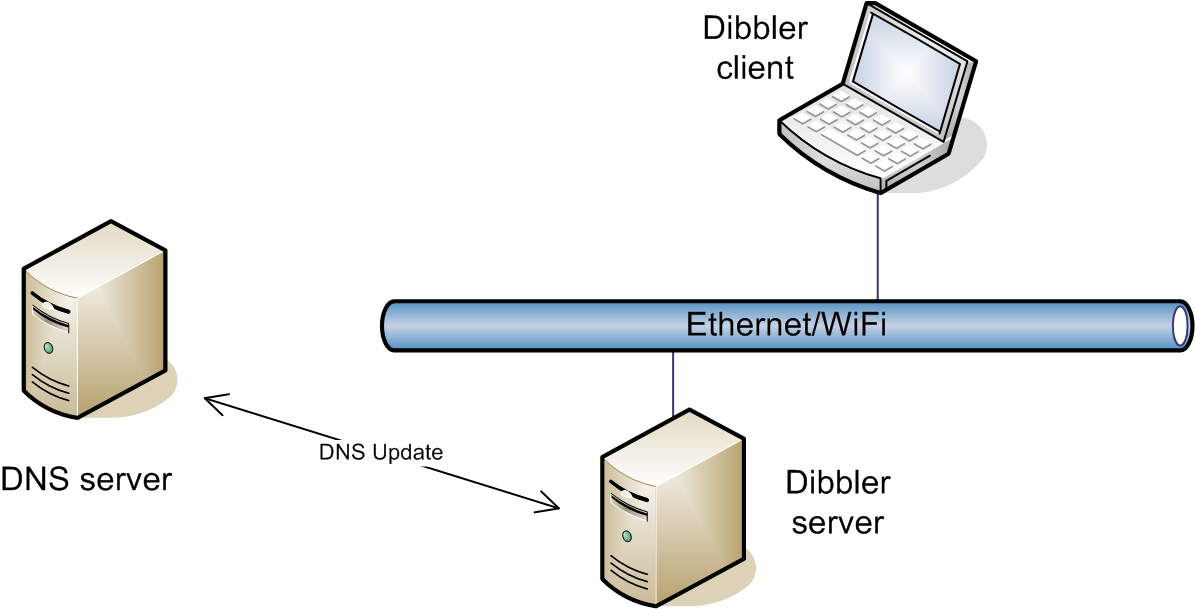
\includegraphics[width=0.65\textwidth]{dibbler-fqdn-srv-update}
\caption{\emph{DNS Update (performed by server)}}
\end{center}
\end{figure}

During normal operation, DHCPv6 client receives one or more IPv6 address(es)
from DHCPv6 server. If configured to do so, it can also receive
information about DNS server addresses. As an additional service, DNS
Update can be performed. This feature, sometimes known as Dynamic DNS,
keeps DNS entries up to date. When client boots, it gets its fully
qualified domain name and this name can be used to reach this
particular client by other nodes. Details of this mechanism is described
in \cite{rfc4704}.

There are two types of the DNS Updates. First is a so called forward
resolving. It allows to change a node's name into its address,
e.g. malcolm.example.com can be translated into 2000::123. Other kind
of record, which can be updated is a so called reverse resolving. It
allows to obtain full name of a node with know address, e.g. 2000::124
can be translated into zoe.example.com.

To configure this feature, following steps must be performed:

\begin{enumerate}
\item Configure DNS server. DNS server supporting IPv6 and dynamic
  updates must be configured. One example of such server is a BIND
  9.3. It is necessary to allow listening on the IPv6 sockets and
  define that specific domain can be updated. See example below.
\item Configure Dibbler server to provide DNS server informations for
  clients. DNS Updates will be sent to the first DNS server on the
  list of available servers.
\item Configure Dibbler server to work in stateful mode, i.e. that it
  can provide addresses for the clients. This is a default mode, so
  unless configuration was altered, this step is already done. Make
  sure that there is no ,,stateless'' keyword in the
  \verb+server.conf+ file.
\item Define list of the available names in the server configuration
  file. Make sure to use fully qualified domain names
  (e.g. malcolm.example.com), not the hostnames only. 
\item Configure dibbler client to request for DNS Update. Use ,,option
  fqdn'' to achieve this. 
\item Server can be configured to execute 
      \begin{itemize}
       \item both (AAAA and PTR) updates by itself
       \item execute PTR only by itself and let client execute AAAA
	     update
       \item don't perform any updates and let client perform AAAA
	     update.
      \end{itemize}
\end{enumerate}

Note that only server is allowed to execute PTR updates. After
configuration, client and/or server should log following line, which
informs that Dynamic DNS Update was completed successfully.

\begin{verbatim}
2006.07.24 01:52:51 Client Notice    FQDN Configured successfully !
\end{verbatim}

\begin{figure}[ht]
\begin{center}
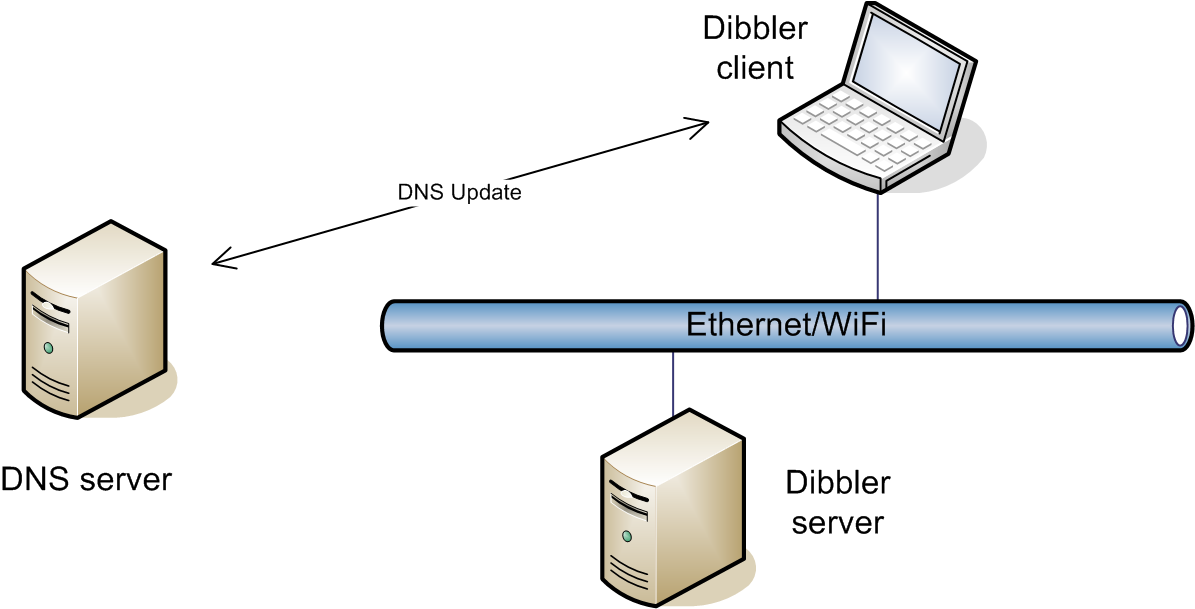
\includegraphics[width=0.65\textwidth]{dibbler-fqdn-cli-update}
\caption{\emph{DNS Update (performed by client)}}
\end{center}
\end{figure}

\subsubsection{Example BIND configuration}
Below are example configuration files for the BIND 9.3. First is a
relevant part of the /etc/bind/named.conf configuration file. Generally,
support for IPv6 in BIND is enabled (listen-on-v6) and there are two
zones added: example.com (normal domain) and
0.0.0.0.0.0.0.0.0.0.0.0.0.0.0.2.ip6.arpa (reverse
mapping). Corresponding files are stored in \verb+example.com+ and
\verb+rev-2000+ files. For details about meaning of those directives,
please consult \emph{BIND 9 Administrator Reference Manual}.

\Note Provided configuration is not safe from the security point of
view. See next subsection for details.
  
\begin{lstlisting}
// part of the /etc/bind/named.conf configuration file
options {
    listen-on-v6 { any; };
    listen-on    { any; };

    // other global options here
    // ...
};

zone "example.com" {
    type master;
    file "example.com";
    allow-update   { any; };
    allow-transfer { any; };
    allow-query    { any; };

    // other example.com domain-specific 
    // options follow
    // ...
};

zone "0.0.0.0.0.0.0.0.0.0.0.0.0.0.0.2.ip6.arpa" {
    type master;
    file "rev-2000";
    allow-update   { any; };
    allow-transfer { any; };
    allow-query    { any; };

   // other 2000::/64 reverse domain related 
   // options follow
   // ...
};
\end{lstlisting}

% \vspace{-0.3cm}
% \begin{center}
% BIND's named.conf example
% \end{center}

Below are examples of two files: forward and reverse zone. First example
presents how to configure normal domain. As an example there is entry
provided for zoe.example.com host, which has 2000::123 address. Note
that you do not have to manually configure such entries -- dibbler will
do this automatically. It was merely provided as an example, what kind
of mapping will be done in this zone.

\begin{lstlisting}
; 
$ORIGIN .
$TTL 86400      ; 1 day
example.com             IN SOA  v13.klub.com.pl. root.v13.klub.com.pl. (
                                129        ; serial
                                7200       ; refresh (2 hours)
                                3600       ; retry (1 hour)
                                604800     ; expire (1 week)
                                86400      ; minimum (1 day)
                                )
                        NS      v13.klub.com.pl.
                        A       1.2.3.4
                        TXT     "Fake domain used for Dibbler tests."
$ORIGIN example.com.
$TTL 7200       ; 2 hours
zoe                     AAAA    2000::123
\end{lstlisting}

Second example presents zone file for reverse mapping. It contains
entries for a special zone called
0.0.0.0.0.0.0.0.0.0.0.0.0.0.0.2.ip6.arpa. This zone represents 2000::/64
address space. As an example there is a static entry, which maps address
2000::999 to a canonical name kaylee.example.com. Note that you do not
have to manually configure such entries -- dibbler will do this
automatically. It was merely provided as an example, what kind
of mapping will be done in this zone.

\begin{lstlisting}
; rev-2000 example file
$ORIGIN .
$TTL 259200     ; 3 days

; this line below is split in two due to page with limitation
0.0.0.0.0.0.0.0.0.0.0.0.0.0.0.2.ip6.arpa IN 
      SOA 0.0.0.0.0.0.0.0.0.0.0.0.0.0.0.2.ip6.arpa. hostmaster.ep.net. (
; this line above is split in two due to page with limitation
                                200608268  ; serial
                                86400      ; refresh (1 day)
                                1800       ; retry (30 minutes)
                                172800     ; expire (2 days)
                                259200     ; minimum (3 days)
                                )
                        NS      klub.com.pl.
$ORIGIN 0.0.0.0.0.0.0.0.0.0.0.0.0.0.0.0.0.0.0.0.0.0.0.0.0.0.0.0.2.ip6.arpa.
$TTL 86200      ; 23 hours 56 minutes 40 seconds
3.2.1                   PTR     picard.example.com.

; this line below is split in two due to page with limitation
9.9.9                   PTR     kaylee.example.com.
$ORIGIN 0.0.0.0.0.0.0.0.0.0.0.0.0.0.0.2.ip6.arpa.

; example entry: 2000::999 -> troi.example.com.
; this line below is split in two due to page with limitation
9.9.9.0.0.0.0.0.0.0.0.0.0.0.0.0.0.0.0.0.0.0.0.0.0.0.0.0.0.0.0.2.ip6.arpa 
      PTR troi.example.com.
; this line above is split in two due to page with limitation
\end{lstlisting}
\Note Due to page width limitation, if the example above, two lines were
split. 
%% $

\subsubsection{Dynamic DNS Testing and tips}
Proper configuration of the DNS Update mechanism is not an easy
task. Therefore this section provides description of several methods of
testing and tuning BIND configuration. Please review following steps
before reporting issues to the author or on the mailing list.

\begin{itemize}
\item See example server and client configuration files described in a
      sections \ref{example-client-fqdn} and \ref{example-server-fqdn}. Also
      note that Dibbler distribution should be accompanied with several
      example configuration files. Some of them include FQDN usage examples.
\item Make sure that unix user, which runs BIND, is able to create and
      write file example.com.jnl. When BIND is unable to create this
      journal file, it will fail to accept updates from dibbler and will
      report failure. Check BIND log files, which are usually stored in the
      \verb+/var/log/+ directory.
\item Make sure that you have routing configured properly on a host,
      which will attempt to perform DNS Update. Use ping6 command to
      verify that DNS server is reachable from this host.
\item Make sure that your DNS server is configured properly. To do so,
      you might want to use \verb+nsupdate+ tool. It is part of the BIND
      distribution, but it is sometimes distributed separated as part of
      the dnsutils package. After executing nsupdate tool, specify
      address of the DNS server (\verb+server+ command), specify update
      parameters (\verb+update+ command) and then type \verb+send+. If
      nsupdate return a command prompt, then the update was
      successful. Otherwise nsupdate will print DNS server's response,
      e.g. NOTAUTH of SRVFAIL. See below for examples of successful
      forward (AAAA record) and reverse (PTR record) updates.
\item After DNS Update is performed, DNS records can be verified using
      dig command line tool (a part of the dnsutils package). Command
      syntax is: 
      \verb+dig @(dns-server-address) name record-type+. 
      In the following example, this query checks for name
      jayne.example.com at a server located at 2000::1 address. Record
      type AAAA (standard record for resolving name into IPv6 address)
      is requested. dig tool provides server's response in the
      \verb+ANSWER SECTION:+. See example log below.
\item In example BIND configuration above, zone transfers, queries and
      updates are allowed from anywhere. To make this configuration more
      secure, it might be a good idea to allow updates only from a
      certain range of addresses or even one (DHCPv6 server's) address
      only.
\end{itemize}


%%%%%%%%%%%%%%%%%%%%%%%%%%%%%%%%%%%%%%%%%%%%%%%%%%%%%%%%%%%%%%%%%%%%%%%%%%%%%%%%

To manually make AAAA record update, type:
\begin{lstlisting}
nsupdate
>server 2000::1
>update add worf.example.com 7200 IN AAAA 2000::567
>send
\end{lstlisting}

To manually make PTR record update, type:
\begin{lstlisting}
nsupdate
>server 2000::1
>update add 
3.2.1.0.0.0.0.0.0.0.0.0.0.0.0.0.0.0.0.0.0.0.0.0.0.0.0.0.0.0.0.2.ip6.arpa.
86200 IN PTR picard.example.com. 
>send
\end{lstlisting}

\Note Everything between "update" and "picard.example.com" must be typed in one line.

And here is an example dig session:

\begin{lstlisting}
v13:/var# dig @2000::1 jayne.example.com AAAA
; <<>> DiG 9.3.2 <<>> @2000::1 jayne.example.com AAAA
; (1 server found)
;; global options:  printcmd
;; Got answer:
;; ->>HEADER<<- opcode: QUERY, status: NOERROR, id: 33416
;; flags: qr aa rd ra; QUERY: 1, ANSWER: 1, AUTHORITY: 1, ADDITIONAL: 2

;; QUESTION SECTION:
;jayne.example.com.             IN      AAAA

;; ANSWER SECTION:
jayne.example.com.      7200    IN      AAAA    2001::e4

;; AUTHORITY SECTION:
example.com.            86400   IN      NS      v13.klub.com.pl.

;; Query time: 6 msec
;; SERVER: 2000::1#53(2000::1)
;; WHEN: Mon Jul 24 01:38:13 2006
;; MSG SIZE  rcvd: 136
\end{lstlisting}
%% >>

\subsection{Server address caching}
Previous Dibbler versions assigned a random address from the available
address pool, so the same client received different address each time it
asked for one. In the 0.5.0 release, new mechanism was introduced
to make sure that the same client gets the same address each time. It is
called \emph{Server caching}.

Below is the algorithm used by the server to assign an address to the client.

\begin{itemize}
 \item if the client provided hint, it is valid (i.e. is part of the
       supported address pool) and not used, then assign requested address.
 \item if the client provided hint, it is valid (i.e. is part of the 
       supported address pool) but used, then assign free address from
       the same pool.
 \item if the client provided hint, but it is not valid (i.e. is not
       part of the supported address pool, is link-local or a multicast
       address), then ignore the hint completety.
 \item if the did not provide valid hint (or provided invalid one), try
       to assign address previously assigned to this client (address caching)
 \item if this is the first time the client is seen, assign any address
       available.
\end{itemize}
%% see SrvOptions/SrvOptIA_NA.cpp, TSrvOptIA_NA::getFreeAddr() method

\subsection{Relays}
\label{features-relays}
In small networks, all nodes (server, hosts and routers) are connected
to the same network segment -- usually Ethernet segment or a single
access point or hotspot. This is very convenient as all clients can
reach server directly. However, larger networks usually are connected
via routers, so direct communication is not always possible. On the
other hand it is useful to have one server, which supports multiple
links -- some connected directly and some remotely.

\begin{figure}[ht]
\begin{center}
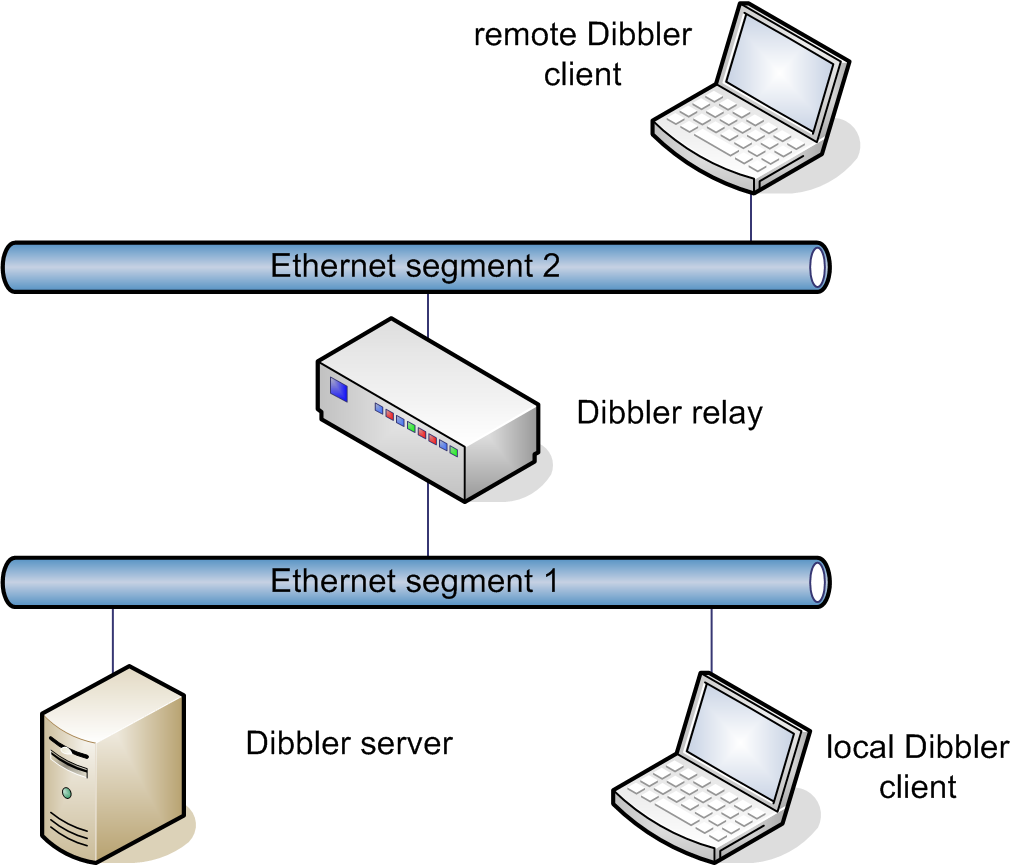
\includegraphics[width=0.65\textwidth]{dibbler-relay}
\caption{\emph{Relay deployment}}
\end{center}
\end{figure}

Very nice feature of the relays is that they appear as actual servers
from the client's point of view. Therefore no special arrangement or
configuration on the client side is required. On the other hand, from
the administrator point of view, it is much easier to manage one DHCPv6
server and deploy several relays than manage several servers on remote
links. 

It is important to understand that relays not simply forward DHCPv6
messages. Each message forwarded from client to the server is
encapsulated. Also each message forwarded from server to a client is
decapsulated. Therefore additional server configuration is required to
deal with encapsulated (i.e. relayed) traffic.

To avoid confusion during reference to a specific link (i.e. eth0 on
the relay may be different link than eth0 on the server), each link
must be referred to using its unique interface-id. For simplicity
reasons, Dibbler uses 4 bytes long identifiers, which are specified as
numbers. It is essential to use the same indentifier in the relay
configuration as well as in the server, so both will refer to the same
link using the same number. See section \ref{example-server-relay1} for
example how to configure server and section \ref{example-relay-1} for 
corresponding relay configuration.

\begin{figure}[ht]
\begin{center}
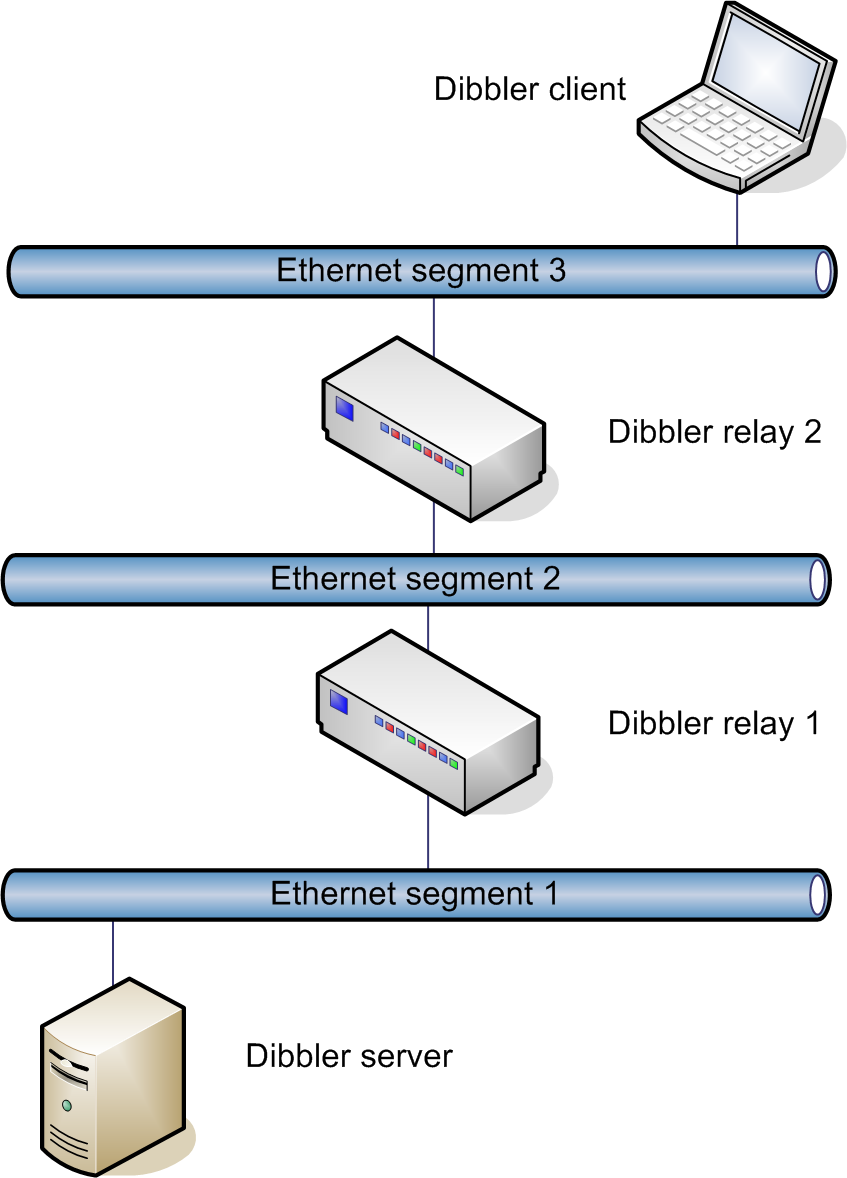
\includegraphics[width=0.4\textwidth]{dibbler-cascade-relays}
\caption{\emph{Cascade relays}}
\label{fig-cascade-relays}
\end{center}
\end{figure}

In larger networks it is sometimes useful to connect multiple
relays. Assuming there are 2 relays connecting server and client. Such
scenario is depicted on figure \ref{fig-cascade-relays}. Requests from
client are received by relay2, which encapsulates and sends them to
relay1. Relay1 further encapsulates those messages and sends them to
the server. Since server receives double encapsulated messages, it
must be properly configured to support such traffic. See section
\ref{example-server-relay2} for details about server configuration and 
section \ref{example-relay-cascade} for example relays configuration.

\subsection{XML files}
\label{features-xml}
During its execution, all dibbler components (client, server and
relay) store its internal information in the XML files. In Linux
systems, they are stored in the \verb+/var/lib/dibbler+ directory. In
Windows, current directory (i.e. directory where exe files are
located) is used instead. There are several xml files generated. Since
they are similar for each component, following list provides
description for server only:

\begin{itemize}
\item server-CfgMgr.xml -- Represents information read from a
  configuration file, e.g. available address pool or DNS server
      configuration.
\item server-IfaceMgr.xml -- Represens detected interfaces in the
  operating system, as well as bound sockets and similar information.
\item server-AddrMgr.xml -- This is database, which contains identity
  associations with associated addresses.
 \item server-cache.xml -- Since caching is implemented by the server
      only, this file is only created by the server. It contains
      information about previously assigned addresses. 
\end{itemize}

\subsection{Prefix delegation}
\label{features-prefix}
According to \cite{rfc3633}: 

\begin{quote}
   The prefix delegation mechanism is
   intended for simple delegation of prefixes from a delegating router
   to requesting routers.  It is appropriate for situations in which the
   delegating router does not have knowledge about the topology of the
   networks to which the requesting router is attached, and the
   delegating router does not require other information aside from the
   identity of the requesting router to choose a prefix for delegation.
   For example, these options would be used by a service provider to
   assign a prefix to a Customer Premise Equipment (CPE) device acting
   as a router between the subscriber's internal network and the service
   provider's core network.
\end{quote}

\begin{figure}[ht]
\begin{center}
\label{fig-prefixes-host}
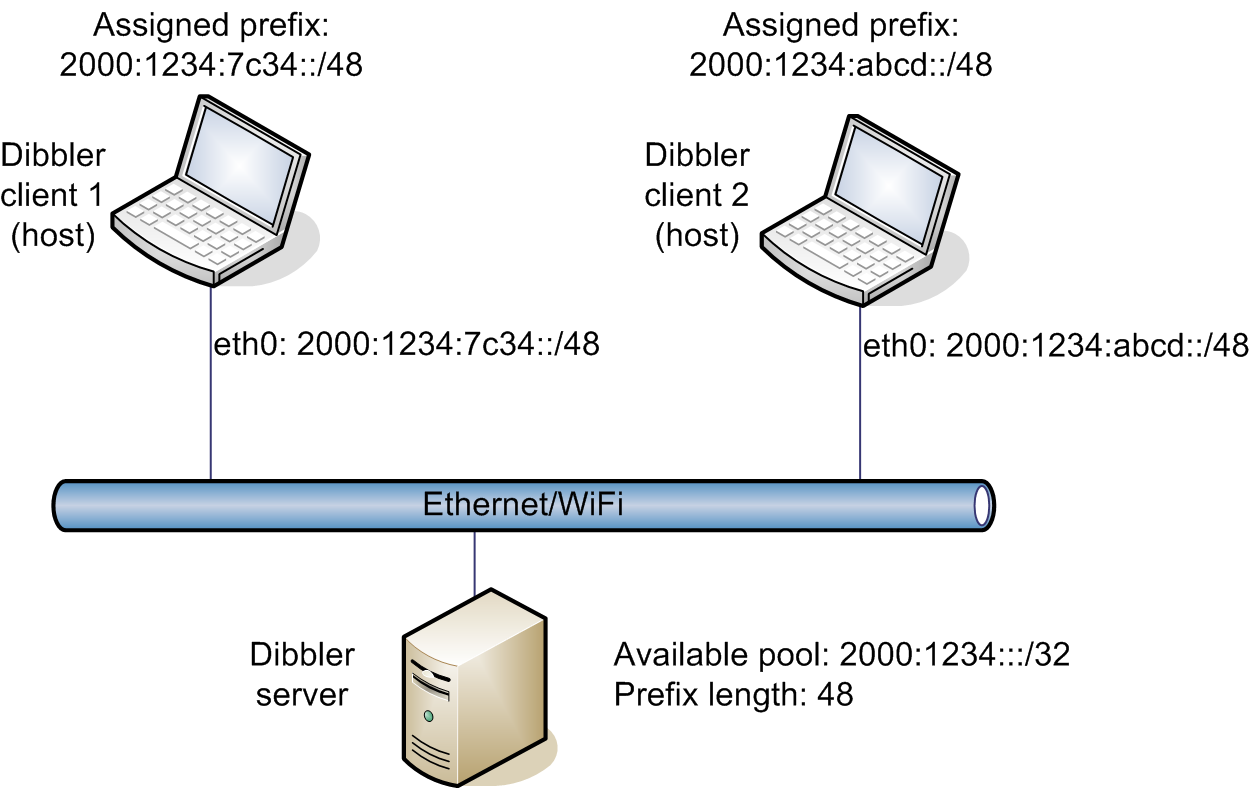
\includegraphics[width=0.65\textwidth]{dibbler-prefixes-host}
\caption{\emph{Prefix delegation (host behaviour)}}
\end{center}
\end{figure}

To configure server to provide prefixes, a pool must be defined and
also client prefixes' length. For example section below assigns
2000:1234::/32 pool to be managed by this server. From this pool,
server will assign /48 prefixes to the clients. For example, client
can receive prefix 2000:1234:7c34::/48. 

\begin{lstlisting}
pd-class {
    pd-pool 2000:1234::/32
    pd-length 48
}
\end{lstlisting}

As a general rule, server will provide random prefix to a client,
unless client provided a hint. The full prefix assignment algorithm is
as follows:

\begin{enumerate}
\item client didn't provide any hints: one prefix from each pool will
  be granted
\item client has provided hint and that is valid (supported and
  unused): requested prefix will be granted
\item client has provided hint, which belongs to supported pool, but this prefix is used:
  other prefix from that pool will be asigned
\item client has provided hint, but it is invalid (not beloninging to
  a supported pool, multicast or link-local): see point 1
\end{enumerate}

Dibbler implementation supports prefix delegation, but it also
extends it. From the server point of view, everything works according
to specs \cite{rfc3633}. However, client is able to meaningfully use
received prefix, even when packet forwarding is not enabled
(i.e. client is a host, not a router). In fact, this is simpler
scenario, therefore it will be explained first. This scenario is
depicted on Fig. \ref{fig-prefixes-host}. When dibbler client receives
prefix and detects that packet forwarding in not enabled, it will
configure received prefix on the interface, which data has been
received on.

Client's behavior is radically different if packet forwarding is
enabled (i.e. client is a router, not a host). In such scenario, when
client receives prefix on one interface (e.g. prefix
2000:1234:7c34::/48 received on eth0) it will generate subprefixes for
all other interfaces, which are up, running, non-loopback and
multicast capable. In the example depicted on
Fig. \ref{fig-prefixes-router}, received prefix was split into 3
prefixes: 2000:1234:7c34:1000::/56 for eth1, 2000:1234:7c34:2000::/56 for eth2
and 2000:1234:7c34:3000::/56 for eth3.

\begin{figure}[ht]
\begin{center}
\label{fig-prefixes-router}
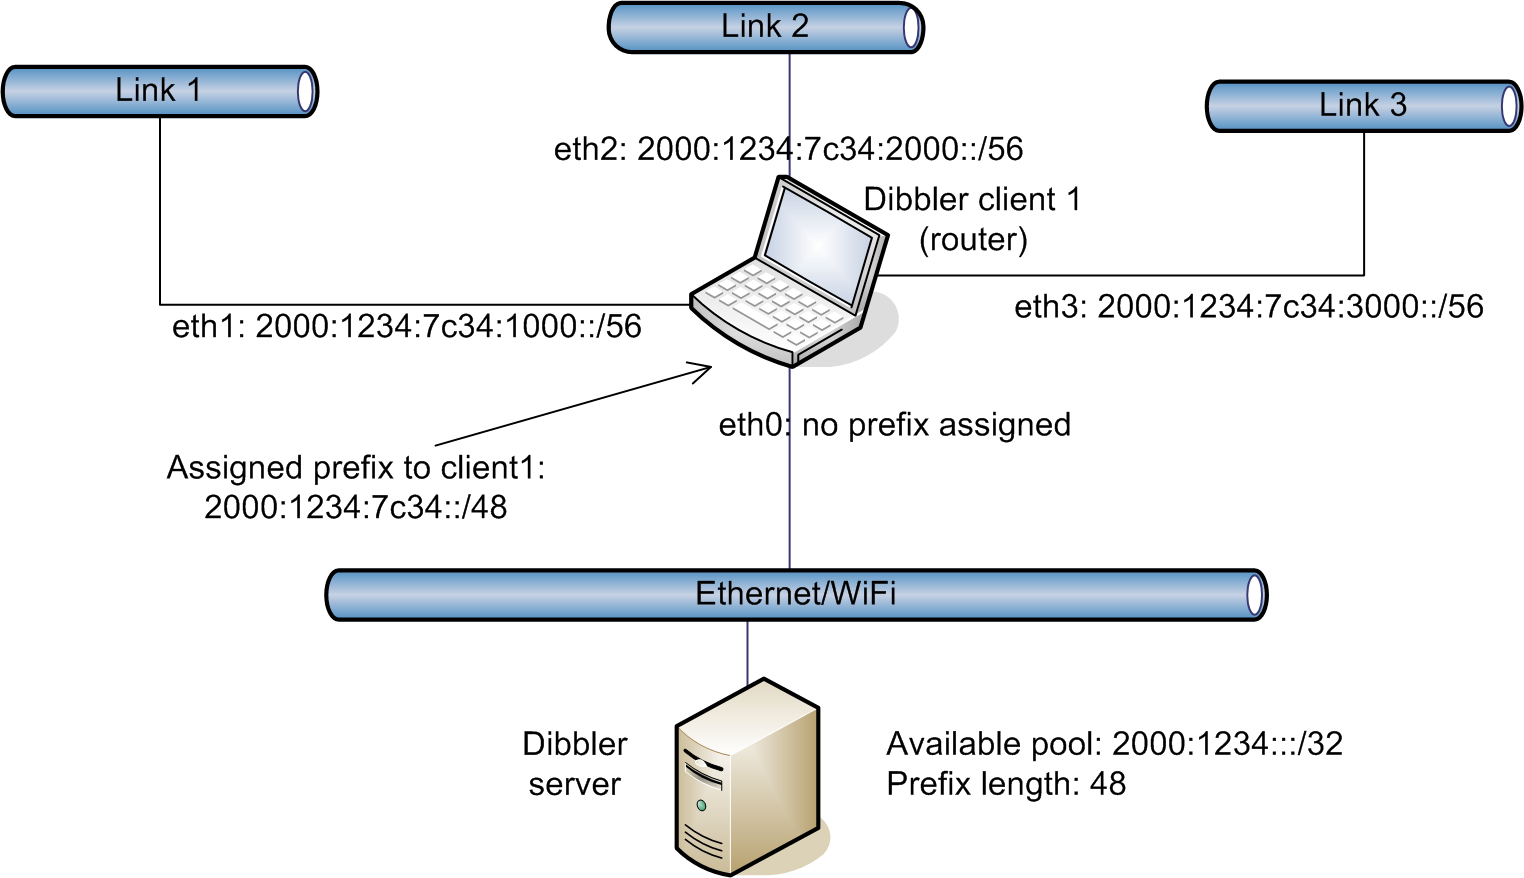
\includegraphics[width=0.65\textwidth]{dibbler-prefixes-router}
\caption{\emph{Prefix delegation (router behaviour)}}
\end{center}
\end{figure}

It is also possible to define multiple prefix pools. See section
\ref{example-server-prefix} for simple prefix delegation configuration
for server or section \ref{example-server-prefixes} for multiple
prefixes configuration. Also section \ref{example-client-prefix}
provides information related to client configuration.

\subsection{Exceptions: per client configuration}
\label{features-exceptions}
All configuration parameters (except FQDN) are the same for all
clients, e.g. all clients will receive the same domain name and the
same DNS servers information. 

However, it is sometimes useful to provide some clients with different
configuration parameters. For example computers from the accouting
department in a corporate network may be configured to be in a
different subdomain. Is is possible to specify that for particular
client different configuration options should be provided. Each client
is identified by its DUID. This mechanism is called \emph{per client
  configuration}, but it is sometimes referred to as \emph{exceptions}.

Note: This mechanism does not apply to address and prefix granting,
because each client receives unique addresses and unique prefixes anyway.

See section \ref{example-server-exceptions} for server configuration examples.

\subsection{Vendor specific information}
Dibbler supports vendor specific information options. As the name
suggests, that option is specific to a particular vendor. To be able
to support any vendor in a flexible manner, values are specified in a
hex format in \verb+server.conf+. For example:

\begin{lstlisting}
 option vendor-spec 1234-0x00002fedc
\end{lstlisting}

When client asks for a vendor-specific info, server will send
vendor-specific info option with enterprise number set to 1234 and
value option-data will be 00002fedc.

Although uncommon, it is also possible to specify multiple vendor
options. Another \verb+server.conf+ example:

\begin{lstlisting}
 option vendor-spec 1234-0x00002fedc,5678-0x0002aaaa
\end{lstlisting}

Server algorithm for choosing, which vendor option should be sent,
works as follows:

\begin{itemize}
\item When client requests for a speficic vendor (i.e. sends
  \opt{vendor-spec info} option with vendor field set), it will
  receive option for that specific vendor (i.e. requested 1234, got 1234).
 \item When client requests any vendor (i.e. sends only \opt{option request} option
   with vendor-spec mentioned), it will receive first \opt{vendor-spec
     info} option from the list (i.e. 5678/0002aaaa).
 \item When client requests for not supported vendor (i.e. 11111), it will    
   receive first vendor-spec option from the list
   (i.e. 5678/0002aaaa).
\end{itemize}

It is possible to configure Dibbler client to ask for vendor-specific
info. Granted value will not be used, so from the client's point of
view this feature may be used as testing tool for the server. Client
can request \opt{vendor-specific information} option in one of the following ways:

\begin{description}
\item[option vendor-spec] -- Only \opt{option request} option will be sent
  with \opt{vendor-spec info} option mentioned.
\item[option vendor-spec 1234] -- \opt{option request} option will be sent
  with \opt{vendor-spec info} option mentioned, but also \opt{vendor-spec
  info} option with enterprise number set to 1234 will be sent.
\item[option vendor-spec 1234 0x0a0b0c0d] -- \opt{option request} option will be sent
  with \opt{vendor-spec info} option mentioned, but also
\opt{vendor-spec info} option with enterprise number set to 1234 and
option-data will be sent.
\end{description}

Although that is almost never needed, it is possible to configure
client to request multiple vendor-specific options at the same
time. That is also supported by the server. See
\ref{example-client-vendor-spec} for examples.


However, if client sends requests for multiple vendor-specific
options, which are not supported by the server, for each sent option,
server will assign one default vendor-spec option.

See \ref{example-client-vendor-spec} for client example and
\ref{example-server-vendor-spec} for server examples.

\subsection{Not connected interfaces (inactive-mode)}
\label{feature-inactive-mode}
During normal startup, client tries to bind all interfaces defined in
a configuration file. If such attempt fails, client reports an error
and gives up. Usually that is best action. However, in some cases it
is possible that interface is not ready yet, e.g. WLAN interface did
not complete association. Dibbler attempt to detect link-local
addresses, bind any sockets or initiate any kind of communication will
fail. To work around this disadvantage, a new mode has been
introduced in the 0.6.0RC4 version. It is possible to modify client
behavior, so it will accept downed and not running interfaces. To do
so, \emph{inactive-mode} keyword must be added to client.conf file. In
this mode, client will accept inactive interfaces, will add them to
inactive list and will periodically monitor its state. When the
interface finally goes on-line, client will try to configure it.

\begin{lstlisting}
#client.conf
inactive-mode

iface wifi0 {
  ia
  option dns-server
}
\end{lstlisting}

To test this mode, you can simulate deassociation using normal
Ethernet interface. Issue following commands:

\begin{itemize}
\item ifconfig eth0 down
\item edit \verb+client.conf+ to enable inactive-mode
\item execute client: \verb+dibbler-client run+
\item client will print information related to not ready interface,
  and will periodically (once in 3 seconds) check interface state.
\item in a separate console, issue \verb+ifconfig eth0 up+ to bring
  the interface up.
\item dibbler-client will detect this and will initiate normal
  configuration process.
\end{itemize}

In the 0.6.1 version, similar feature has been introduced on the
server side.

\subsection{Parameters not supported by server (insist-mode)}
\label{feature-insist-mode}

Client can be instructed to obtain several configuration options, for
example DNS server configuration or domain name. It is possible that server
will not provide all requested options. Older versions of
the dibbler client had been very aggressive in such case. It tried
very hard to obtain such options. To do so, it did send
\msg{INF-REQUEST} to obtain such option. It is possible that some
other DHCPv6 servers will receive this message and will reply with
valid configuration parameters. This behavior has
changed in the 0.6.0RC4 release. Right now when client does not
receive all requested options, it will complain, but will
take no action. To enable old behavior, so called insist-mode has been
added. To enable this mode, add \verb+insist-mode+ at the global
section of the \verb+client.conf+ file. For example:

\begin{lstlisting}
log-mode short
insist-mode

iface eth0 {
   ia
   option dns-server
   option domain
   option ntp-server
}


\end{lstlisting}

\subsection{Different DUID types}
\label{feature-duid-types}
There are 3 different types of the DUID (DHCP Unique Identifier):
\begin{itemize}
\item type 1 (link-layer + time) -- this DUID is based on Link-layer
  address and a current timestamp. According to spec \cite{rfc3315},
  that is a default type.
\item type 2 (enterprise number) -- this DUID is based on the Private
  Enterprise Number assigned to larger companies. Each vendor should
  maintain its own space of unique identifiers.
\item type 3 (link-layer) -- this DUID is based on link-layer address
  only.
\end{itemize}

According to spec \cite{rfc3315}, it is recommended to use link-layer
+ time, if possible. That DUID type provides most uniqueness. It has
one major drawback -- it is impossible to know DUID before it is
actually generated. That poses significant disadvantage to sysadmins,
who want to specify different configuration for each client. In such
cases, it is recommended to switch to link-layer only (type 3) DUIDs.

During first executing dibbler-client will generate its DUID and store
it in \verb+client-duid+ file on disk. During next startup DUID will
be read from the file, not generated. 

It is possible to specify, what DUID format should be used. It is
worth noting that such definition is taken into consideration during
DUID generation only, i.e. during first client execution. To specify
DUID type, put only one of the following lines in the
\verb+client.conf+ file:

\begin{lstlisting}

# uncommend only ONE of the lines below
duid-type duid-llt
#duid-type duid-en 1234 0x56789abcde
#duid-type duid-ll

iface eth0 {
   ia
   option dns-server
}
\end{lstlisting}

When using link-layer+time or link-layer DUID types, dibbler will
autodetect addresses. To generate enterprise number-based DUID,
specific data must be provided: enterprise-number (a 32-bit integer,
1234 in the example above) and a enterprise-specific indentifier of
arbitrary length (56:78:9a:bc:de in the example above).

\subsection{Debugging/compatibility features}
During interoperability test session, it has been discovered that
sometimes various different implementations of the DHCPv6 protocol has
problem to interact with each other. As the protocol itself does not
specify all aspects and details, some things can ba done differently
and there is no only one ,,proper way''. It also happens that some
implementations may have problems with different than its authors
expected behaviors. To allow better interoperation between such
implementation, dibbler has some features, which cause different
behaviors. This could result in a successful operation with other
servers, clients and relays.

Normal users don't have to worry about those options, unless they are
using different servers, clients and relays. Those options also may be
useful for other vendors, who want to test their
implementations. Therefore those options can be perceived as a
debugging or testing features.

\subsubsection{Interface-id option}

During message relaying (done by relays), options can be placed in the \msg{RELAY-FORW}
message is arbitrary order. In general, there are two options used:
\opt{interface-id} option and \opt{relay-message} option. The former
defines interface identifier, which the original data has been
received from, while the later contains the whole original
message. When several relays are used, such message-in-option
encapsulation can occur multiple times.

It is possible to instruct relay to store \opt{interface-id} before
\opt{relay-message} option or after. There is also possibility to instruct
server to omit the \opt{interface-id} option altogether, but since 
this violates \cite{rfc3315}, it should not be used. In general, this
configuration parameter is only useful when dealing with buggy relays,
which can't handle all option orders properly. Consider this parameter
a debugging feature.

Similar parameter is defined for the server. Server uses it during
\msg{RELAY-REPL} generation. 

See description of the \emph{interface-id-order} parameters in Server
configuation (section \ref{server-conf}) and Relay configuration
(section \ref{relay-conf}).

\subsubsection{Non-empty IA\_NA option}
When client is interested in receiving an address, it sends
\opt{IA\_NA} option. In this option it may (but don't have to) include
addresses (using \opt{IAADDR} suboption) as hints for the server.

It has been detected that some servers does not support properly
(perfectly valid) empty \opt{IA\_NA} options. To work around this
problem, dibbler-client can be instructed to include \opt{IAADDR} in
the \opt{IA\_NA} option. Here is minimal example config. file, which
achieves that:

\begin{lstlisting}
iface eth0 {
  ia {
     address
  } 
}
\end{lstlisting}

\subsection{Experimental features}

This section contains experimental features. Besides serving as a
general purpose DHCPv6 solution, dibbler is also used as a research
tool for new ideas. \footnote{Since my (Tomasz Mrugalski) Ph.D finally
started to take shape, some of my research topics will be examined and
verified in the dibbler.} Normal users are recommended NOT to use any
of those features. Advanced users should take extra caution. Also be
aware that those options may not work as expected, may be incomplete
and not documented properly. You have been warned.

Since those mechanisms are non-standard, they are disabled by
default. To enable them, ,,experimental'' keyword must be placed in
the \verb+client.conf+ or \verb+server.conf+ files.

\subsubsection{Address Parameters}

\textbf{Note: This feature is experimental, i.e. it is not described
by any RFC or even internet draft. Don't use it, unless you exactly
know what you are doing.}

There is ongoing process to register and publish internet draft,
which describes this operation. Latest versions of this draft will be
availabe at \url{http://klub.com.pl/dhcpv6/doc/}.

RFC3315 (\cite{rfc3315}) defines means of allocating IPv6 addresses to
all interested clients. Clients are able to obtains IPv6 addresses and
other configuration parameters from the servers. Unfortunately, client
after obtaining an address, are not able to communicate each other due
to missing prefix information. That property of the DHCPv6 procotol is
sometimes perceived as a major disadvantage. To overcome this
deficiency, an extension to the protocol has been proposed.

It is possible to attach additional option conveyed in normal IAADDR
option. That additional option, called ADDRPARAMS option, contains
additional information related to that address. To maintain backward
compatibility, server does not send such option by default, even when
configured to support it. To make server send this option, client must
explicitly ask for it. 

Below are example configuration files for server and client. Note that
since that is an non-standard feature, user must explicitly allow
experimental options before configuring it (thus ,,experimental''
keyword is required).

Example \verb+client.conf+ configuration file:

\begin{lstlisting}
#client.conf
log-mode short
log-level 8


iface "eth0" {
  ia { 
     addr-params 
  }
}
\end{lstlisting}

Example \verb+server.conf+ configuration file:

\begin{lstlisting}
#server.conf
log-level 8

experimental
log-mode short

iface eth0 {

 t1 60
 t2 96
 prefered-lifetime 120
 valid-lifetime 180

 class {
   addr-params 80
   pool 2001:458:ff01:ff03::/80
 }
}
\end{lstlisting}


%% CONFIG FILES
%%
%% Dibbler - a portable DHCPv6
%%
%% authors: Tomasz Mrugalski <thomson@klub.com.pl>
%%
%%
%% released under GNU GPL v2 licence
%%
%% $Id: dibbler-user-config.tex,v 1.26 2006-09-04 01:28:35 thomson Exp $
%%

\section{Configuration files}

This section describes Dibbler server, relay  and client
configuration. Square brackets denotes optional values: mandatory
[optional]. Alternative is marked as $\mid$. A $\mid$ B means A or
B. Parsers are case-insensitive, so Iface, IfAcE, iface and IFACE mean
the same. This does not apply to interface names. eth0 and
ETH0 are dwo diffrent interfaces.

\subsection{Tokens and basic informations}
Config file parsing is token-based. Token can be considered a keyword
or a specific phrase. Here's list of tokens used:
\begin{description}
\item[IPv6 address] -- IPv6 address, e.g. 2000:dead:beef::789
\item[32-bit decimal integer] -- string containing only numbers, e.g. 123456
\item[string] -- string of arbitrary characters enclosed in single or double
  quotes, e.g. 'this is a string'. If string contains only a-z, A-Z and
  0-9 characters, quotes can be omited, e.g. beeblebrox
\item[DUID identifier] -- hex number starting with 0x, e.g. 0x12abcd.
\item[IPv6 address list] -- IPv6 addresses separated with commas,
	   e.g. 2000::123, 2000::456
\item[DUID list] -- DUIDs separated with commas, e.g. 0x0123456,0x0789abcd
\item[string list] -- strings separated with comas, e.g. tealc,jackson,carter,oneill
\item[boolean] -- YES, NO, TRUE, FALSE, 0 or 1. Each of them can be
  used, when user must enable or disable specific option.
\end{description}

\subsection{Scopes}
There are four scopes, in which options can be specified: global,
inteface, IA and address. Every option is specific for one scope.
Each option is only applied to a scope and all subscopes in which it is
defined.

For example, T1 is defined for
IA scope. However, it can be also used in more common scopes. In this
case -- in interface or global. Defining T1 in interface scope means:
,,for this interface default value for T1 is ...''. The same applies
to global scope. Options can be used multiple times. In that case
value defined later is used.

Global scope is the largest. It covers the whole config file and
applies to all intefaces, IAs, and addresses, unless some lower scope
options override it. Next comes inteface scope. Options defined there
are inteface-specific and apply to this interface, all IAs in this
interface and addresses in those IAs. Next is IA scope. Options
defined there are IA-specific and apply to this IA and to addresses it
contains. Least significant scope is address. 

\subsection{Comments}

Comments are also allowed. All common comment styles are supported:
\begin{itemize}
\item C++ style one-line comments: // this is comment
\item C style multi-line comments: /* this is multiline comment */
\item bash style one-line comments: \# this is one-line comment
\end{itemize}

\subsection{Client configuration file}

Client configuration file should be named \verb+client.conf+. It should be
placed in the \verb+/etc/dibbler/+ directory (Linux system) or in the
current directory (Windows systems). After successful startup, old
version of this file is stored as \verb+client.conf-old+. One of
design requirements for client was ,,out of the box'' usage. To
achieve this, simply use empty 
\verb+client.conf+ file. Client will try to get one address for each up and
running interface \footnote{Exactly: Client tries to configure each
  up, multicast-capable and running interface, which has link address
  at least 6 bytes long. So it will not configure tunnels (which
  usually have IPv4 address (4bytes long) as their link address. It
  should configure all Ethernet and 802.11 interfaces. The latter was
  not tested by author due to lack of access to 802.11 equipment.}.

\subsubsection{Global parameters}

There are several global options. Those options can be used in the
global scope. However, inteface, IA and address scoped options can be
used in the global scope, too. 
Client configuration file has following syntax:

\begin{verbatim}
global-options
interface-options
IA-options
address-options
interface-declaration
\end{verbatim}

\subsubsection{Interface declaration}

Each system interface, which should be configured, must be mentioned in
the configureation file. Interfaces can be declared with this syntax:
\begin{verbatim}
iface interface-name
{
  interface-options
  IA-options
  address-options        
}
\end{verbatim}

or 

\begin{verbatim}
iface interface-number 
{
  interface-options
  IA-options
  address-options        
}
\end{verbatim}

In the latter case, interface-number denotes interface number. It can be extracted
from ,,ip~l'' (Linux) or
,,ipv6~if'' (Windows). \verb+interface-name+ is an interface
name.  Name of the interface does not have to be enclosed in single or
double quotes. It is necessary only in Windows systems, where interface
names sometimes contain spaces, e.g. ''local network connection''.

Interface scoped options can be used here. IA-scoped as well as address
scoped options can also be used. They will be treated as a default
values for future definitions of the IA and address instantations.

\subsubsection{IA declaration}
IA is an acronym for Identity Association. It is a logical entity
representing address or addresses used to perform some
functions. IA-options can be defined, e.g. T1. IPv6 addresses can be
defined here. All those values will be used as hints for a server.

Almost always, each DHCPv6 client will have exactly one IA on each
interface. IA is declared using following syntax:

\begin{verbatim}
ia
{ 
  IA-options
  address-options
  address-declaration
}
\end{verbatim}

It is also possible to define multiple IA at once. To do so, following
syntax might be used:

\begin{verbatim}
ia number
{ 
  IA-options
  address-options
  address-declaration
}
\end{verbatim}
Number is an optional number, which describes how many such IAs
should be requested. Number is optional. If it is not specified, 1 is
used. If this number is not equal 1, then address options are not
allowed. That could come in handy when someone need serveral IAs with
the same parameters. If IA contains no addresses, client assumes that
one address should be configured.

IA scoped as well as address options can be defined here. IA scoped
options will be applied directly, while address scoped options will be
used as default values for all addresses that will be defined in this
IA. 

\subsubsection{Address declaration}
When IA is defined, it is sometimes useful to define its address. Its
value will be used as a hint for the server.

Address is declared in the following way:

\begin{verbatim}
address number
{ 
  address-options
  IPv6-address
}
\end{verbatim}
where number denotes how many addresses with those values should be
requested. If it is diffrent than 1, then IPv6 address options are not
allowed.

Only address scoped options can be used here.

\subsubsection{Standard options}
So called standard options are defined by the basic DHCPv6
specification, a so called RFC 3315 \cite{rfc3315}. Those options are
called standard, because all DHCPv6 implementations, should properly
handle them. Standard options are declared in the following way:

\begin{verbatim}
OptionName option-value
\end{verbatim}

Every option has a scope it can be used in, default value and
sometimes allowed range. 

\begin{description}
 \item[work-dir] -- (scope: global, type: string, default: .) Defines working
	    directory.
 \item[log-level] -- (scope: global, type: integer, default: 7) Defines
	    verbose level of the log messages. The valid range if
	    from 1 (Emergency) to 8 (Debug). The higher the logging
	    level is set, the more messages dibbler will print.
 \item[log-name] -- (scope: global, type: string, default: Client). Defines 
	    name, which should be used during logging.
 \item[log-mode] -- (scope: global, type: short, full or precise,
	    default value: full) Defines logging mode. In the
	    default, full mode, name, date and time in the h:m:s format
	    will be printed. In short mode, only minutes and
	    seconds will be printed (this mode is useful on
	    terminals with limited width). Recently added precise
	    mode logs information with seconds and microsecond
	    precision. It is a useful for finding bottlenecks in
	    the DHCPv6 autoconfiguration process.
 \item[strict-rfc-no-routing] -- (scope: global, type: none, default:
	    not defined). During normal operation, DHCPv6 client
	    should add IPv6 address only, without configuring
	    routing, because this should be done with other means,
	    i.e. router advertisements \cite{rfc2461}. However,
	    this behavior is confusing and lots of users complained
	    about it, so since the 0.5.0-RC1 release, this has been changed
	    in dibbler. Right now when dibbler client configures
	    address, it also configures routing, so every host is
	    able to communicate with other hosts, which have
	    obtained address from the same server. If you don't
	    like this behavior, you might want to use this option.
 \item[rapid-commit] -- (scope: interface, type: boolean, default:
	    0). This option allows rapid commit procedure to be
	    performed. Note that enabling rapid commit on the client
	    side is not enough. server must be configured to allow
	    rapid commit, too.
 \item[unicast] -- (scope: interface, type: boolean, default: 0). This
	    option specifies if client should request unicast
	    communication from the server. If server is configured to
	    allow it, it will add unicast option to its replies. It will
	    allow client to communicate with server via unicast
	    addresses instead of usual multicast.
 \item[prefered-servers] -- (scope: interface, type: address or duid list, default:
	    empty). This list defines, which servers are prefered. When
	    client sends \msg{SOLICIT} message, all servers available in
	    the local network will respond. When client receives
	    multiple \msg{ADVERTISE} messages, it will choose those sent
	    by servers mentioned on the perfered-server list.
 \item[reject-servers] -- (scope: interface, type: address or duid list, default:
	    empty) This list defines which server must be ignored. It
	    has negative meaning to the prefered-servers list.
 \item[T1] -- (scope: IA, type: integer: default: $2^{32}-1$). This value
	    defines after what time client should start renew
	    process. This is only a hint for the server. Actual value
	    will be provided by the server.
 \item[T2] -- (scope: IA, type: integer, default:$2^{32}-1$). This value
	    defines after what time client will start emergency rebind
	    procedure if renew process fails. This is only a hint for
	    the server. Actual value will be provided by the server.
 \item[valid-lifetime] -- (scope:address, type: integer,
	    default:$2^{32}-1$) This parameter defines valid lifetime of
	    an address. It will be used as a hint for a server, when the
	    client will send requests.
 \item[prefered-lifetime] -- (scope:address, type: integer,
	    default:$2^{32}-1$) This parameter defines prefered lifetime
	    of an address. It will be used as a hint for a server, when
	    there client will send requests.
\end{description}

\subsubsection{Addional options}
Additional options are the options specified in external drafts and in RFC
documents. They are declared with \verb+option+ keyword:

\begin{verbatim}
option OptionName option-value
\end{verbatim}

where OptionName is one of possible values listed below:

\begin{center}
\begin{tabular}{|c|c|>{\centering}p{1.7cm}<{}|c|p{6cm}|}
\hline
OptionName     & Scope    & Values      &default& Description \\
               &          & (default)   &       & \\
\hline
dns-server     & interface& addrs list  & not defined & preferred DNS servers list (H) \\
domain         & interface&domains list & not defined & preferred domain (H)\\
ntp-server     & interface& addrs list  & not defined & preferred NTP servers list (H)\\
time-zone      & interface& timezone    & not defined & preferred time zone (H)\\
sip-server     & interface& addrs list  & not defined & preferred SIP servers list (H)\\
sip-domain     & interface&domains list & not defined & preferred SIP domain (H)\\
nis-server     & interface& addrs list  & not defined & preferred NIS servers list (H)\\
nis-domain     & interface& domain      & not defined & preferred NIS domain (H)\\
nis+-server    & interface& addrs list  & not defined & preferred NIS+ servers list (H)\\
nis+-domain    & interface& domain      & not defined & preferred NIS+ domain (H)\\
lifetime       & interface& YES/NO      & no    & Should client request lifetime option? \\
\hline
\end{tabular}
\end{center}

Note that timezone format is described in file \verb+draft-ietf-dhc-dhcpv6-opt-tz-00.txt+
and domain format is described in RFC 3646. After receiving options
values from a server, client stores them in separate files in the
working directory, e.g. \verb+option-dns-server+. Several options
are processed and set up in the system. Options supported in Linux and
Windows environments are presented in the table below.

\begin{center}
\begin{tabular}{|l|l|l|l|}
\hline
Option & Linux & WinXP/2003 & WinNT/2000  \\
\hline
dns-server  & system, file & system, file & system,file \\
domain      & file         & system, file & file \\
ntp-server  & file         & file & file \\
time-zone   & file         & file & file \\
sip-server  & file         & file & file \\
sip-domain  & file         & file & file \\
nis-server  & file         & file & file \\
nis-domain  & file         & file & file \\
nis+-server & file         & file & file \\
nis+-domain & file         & file & file \\
\hline
\end{tabular}
\end{center}

\subsubsection{Stateless configuration}

If interface does not contain \verb+IA+ keyword, one IA with one address is
assumed. If client should not request for address on this interface,
\opt{stateless}\footnote{In the version 0.2.1-RC1 and earlier, this
  directive was called no-ia. This depreciated name is valid for now,
  but might be removed in future releases.}
must be used. In such circumstances, only specified options will be
requested.

\subsubsection{Relay support}
Usage of the relays is not visible from the client's point of view:
Client can't distinguigh if it communicates via relay(s) or directly
with the server. Therefore no special directives on the client side 
are required to use relays. 

\subsection{Client configuration examples}
This subsection contains various examples of the most configurations.
If you are interested in additional examples, download source version
and look at \verb+*.conf+ files.

\subsubsection{Example 1: Default}

In simplest case, client config can be empty. Client will try to
assign one address for every interface present in the system, except
interfaces:
\begin{itemize}
\item which are down (flag UP not set)
\item loopback (flag LOOPBACK set)
\item which are not running (flag RUNNING not set)
\item which are not multicast capable (flag MULTICAST not set)
\end{itemize}

If you must use DHCPv6 on one of such interfaces (which is not
recommended and probably will fail), you must explicitly specify this
interface in config file.

\subsubsection{Example 2: DNS}

Simple config config file requesting 1 address and DNS configuration
on eth0 interface looks like that:
\begin{Verbatim}
# client.conf
log-mode short
log-level 7
iface eth0 {
  option dns-server
  ia
}
\end{Verbatim}

\subsubsection{Example 3: Timeouts and specific address}

Another example is presented below. Client asks for 1 address and
would like it to be 2000::1:2:3. Rapid-commit is allowed and client
would like to renew this address once in a 10 minutes.

\begin{Verbatim}
# client.conf
log-mode short
log-level 7
iface eth0 {
  T1 1800
  T2 2000
  prefered-lifetime 3600
  valid-lifetime 7200
  rapid-commit YES
  ia {
    address { 
      2000::1:2:3
    }
  }
}
\end{Verbatim}

\subsubsection{Example 4: Unicast, more than one address}

Here's yet another example. We would like to obtain 2 addresses on
,,Local Area Connection'' interface. Note quotation marks around
interface name. They're necessary since this particular interface name
contains spaces. Client also would like to accept Unicast
communication if server supports it. We don't care for
details, so keep those log very short. Take note that you won't be
able to what Dibbler is doing with such low log-level. (Preferred
log-level is 7). Config file looks like that:

\begin{Verbatim}
# client.conf
log-mode short
log-level 5
iface "Local Area Connection" {
  unicast yes
  ia 2
}
\end{Verbatim}

\subsubsection{Exmaple 5: Rapid-commit}
Rapid-commit is a shortened exchange with server. It consists of only
two messages, instead of the usual four. Instead of using interface
name, we provide its index. It is worth to know that server must also 
support rapid-commit.

\begin{Verbatim}
# client.conf
iface 3 {
  rapid-commit yes
  ia 
  option dns-server
}
\end{Verbatim}

\subsubsection{Example 6: Stateless mode}
Client can be configured to work in a stateless mode. It means that it
will obtain only some configuration parameters, but no
addresses. Let's assume we want all the details and we want to obtain
all possible configuration parameters. Here is a configuration file:

\begin{Verbatim}
# client.conf
log-level 8
log-mode full
stateless
iface eth0
{
  option dns-server
  option domain
  option ntp-server
  option time-zone
  option sip-server
  option sip-domain
  option nis-server
  option nis-domain
  option nis+-server
  option nis+-domain
}
\end{Verbatim}

\subsubsection{Example 7: Dynamic DNS (FQDN)}
\label{example-client-fqdn}
Dibbler client is able to request fully qualified domain name,
i.e. name, which is fully resolvable using DNS. After receiving such
name, it can perform DNS Update procedure. Client can ask for any
name, without any preferrence. Here is an example how to configure
client to perform such task:
\begin{Verbatim}
# client.conf
log-level 7
iface eth0 {
# ask for address
    ia

# ask for options
   option dns-server
   option domain
   option fqdn
}
\end{Verbatim}
In this case, client will mention that it is interested in FQDN by
using Option Request. Server upon receiving such request (if it is
configured to support it), will provide FQDN option containing domain
name.

It is also possible for client to provide its name as a hint for
server. Server might take it into consideration when it will choose a
name for this client. Example of a configuration file for such
configuration is provided below:

\begin{Verbatim}
# client.conf
log-level 7
iface eth0 {
# ask for address
    ia

# ask for options
   option dns-server
   option domain
   option fqdn zoe.example.com
}
\end{Verbatim}

Note that to successfully perform DNS Update, address must be assigned
and dns server address must be known. So ,,ia'' and ,,option
dns-server'' is required for ,,option fqdn'' to work properly. Also if
DHCPv6 server provides more than one DNS server addresses, update will
be attempted only to the first one on the list.

\subsection{Server configuration file}

Server configuration is stored in \verb+server.conf+ file in the
+/etc/dibbler+ (Linux systems) or in current (Windows systems)
directory. After successful startup, old version of this file is stored as
\verb+server.conf-old+.

\subsubsection{Global scope}

Every option can be declared in global scope.
Config file has this form:

\begin{verbatim}
 interface declaration  |
 global options         |
 interface options      |
 class options          
\end{verbatim}

\subsubsection{Interface declaration}

Interface can be declared this way:
\begin{verbatim}
iface name_of_this_interface
{
  interface options      |
  class options        
}
\end{verbatim}

or 

\begin{verbatim}
iface number 
{
  interface options      |
  class options        
}
\end{verbatim}

where name\_of\_this\_interface denotes name of the interface and
number denotes it's number. It no longer needs to be enclosed in
single or double quotes (except windows cases, when interface name
contains spaces).

\subsubsection{Class scope}
Address class is declared as follows:

\begin{verbatim}
class
{  
     class options |
     address pool    
}
\end{verbatim}

address pool can be defined in one of the following formats:
\begin{verbatim}
pool minaddress-maxaddress
pool address/prefix
\end{verbatim}

\subsubsection{Options}

Every option has a scope it can be used in, default value and
sometimes allowed range.

%% FIXME: this table must be sanitized
\begin{tabular}{|c|c|>{\centering}p{1.7cm}<{}|c|p{6cm}|}
\hline
Name             & Scope   & Values      & default    & Description \\
                 &         & (default)   &  & \\
\hline
work-dir         & global  & string      & empty      & working directory \\
log-level        & global  & 1-8         & 8          & log-level (8 is most verbose) \\
log-name         & global  & string      & Client     & Name, which appears in a log file\\
cache-size       & global  & integer     & 1048576    & size of the
address cache, specified in bytes \\

preference       &interface& 0-255       & 0          & server preference value (higher is more prefered) \\
unicast          &interface& address     & empty      & Specify which address should be used. \\
iface-max-lease  &interface& integer     & 4294967296 & how many addresses can be leased by all clients? \\
client-max-lease &interface& integer     & 4294967296 & how many addresses can be leased by one client? \\
rapid-commit     &interface& 0 or 1      & 0          & should we allow Rapid Commit (SOLICIT--REPLY)? \\
relay            &interface& string      & not defined& Name of the physical interface used to reach this relay \\
interface-id     &interface& integer     & not defined& ID of the relay interface. Must be unique \\

valid-lifetime   & class   & integer     & 4294967296 & valid lifetime for address (specified in seconds)\\
prefered-lifetime& class   & integer     & 4294967296 & after this amount of time(in seconds) address becomes depreciated\\
T1               & class   & integer     & 4294967296 & client should renew addresses after T1 seconds \\
T2               & class   & integer     & 4294967296 & client should send REBIND after T2 seconds\\
reject-clients   & class   & addrs or 
                             DUID list   & empty      & list containing servers which should be discarded in configuration of this IA \\
accept-only      & class   & addrs or
                             DUID list   & empty      & these are the only clients allowed to use this class\\
class-max-lease  & class   & integer     & 4294967296 & how many addresses can be leased from this class? \\
\hline
\end{tabular}

\begin{itemize}
\item[log-mode] -- defines logging level. Currently supported options
  are: full (daemon name, date and time), short (minutes and seconds), precise
  (seconds and microseconds, used mainly for finding bottlenecks). In
  future releases, syslog (unix only) and eventlog (windows only) will
  be supported. Default is full.
\end{itemize}

\subsubsection{Addional options}
Server supports additonal options, not specified in RFC3315. They have
generic form:

\begin{verbatim}
option OptionName OptionsValue
\end{verbatim}

All supported options are specified in the table below:

\begin{center}
\begin{tabular}{|l|l|c|c|l|}
\hline
OptionName       & OptionsValue& Default    & Description \\ \hline
dns-server       & addrs list  & empty      & DNS servers list \\
domain           & string list & empty      & domain names list \\
ntp-server       & addrs list  & empty      & NTP servers list \\
time-zone        & timezone    & empty      & time zone \\
sip-server       & addrs list  & empty      & SIP servers list \\
sip-domain       & string list & empty      & domain names list \\

nis-server       & addrs list  & empty      & NIS servers list \\
nis-domain       & string      & empty      & domain name \\

nisplus-server   & addrs list  & empty      & NIS+ servers list \\
nis-domain       & string      & empty      & domain name \\
lifetime         & integer     & empty      & how often renew options? \\
\hline
\end{tabular}
\end{center}

Lifetime is a special case. It is not set up by client in a system
configuration. It is, however, used by the client to know how long
obtained values are correct.

\subsection{Server configuration examples}

This subsection contains various examples of the server
configuration. If you are interested in additional examples, download source version
and look at \verb+*.conf+ files.


\subsubsection{Example 1: Simple}

In opposite to client, server uses only interfaces described in config
file. Let's examine this common situation: server has interface
named \emph{eth0} (which is fourth interface in the system) and is
supposed to assign addresses from 2000::100/124 class. Simplest config
file looks like that:

\begin{Verbatim}
# server.conf
iface eth0
{ 
  class
  {
    pool 2000::100-2000::10f
  } 
}
\end{Verbatim}

\subsubsection{Example 2: Timeouts}
Server should be configured to deliver specific timer values to the
clients. This example shows how to instruct client to renew (T1 timer) 
addresses one in 10 minutes. In case of problems, ask other servers in
15 minutes (T2 timer), that allowe prefered lifetime range is from 30
minutes to 2 hours, and valid lifetime is from 1 hour to 1 day. DNS
server parameter is also provided. Lifetime option is used to make
clients renew all non-address related options renew once in 2 hours.

\begin{Verbatim}
# server.conf
iface eth0 
{
  T1 600
  T2 900
  prefered-lifetime 1800-3600
  valid-lifetime 3600-86400
  class
  {
    pool 2000::100/80
  } 

  option dns-server 2000::1234
  option lifetime 7200
}
\end{Verbatim}

\subsubsection{Example 3: Limiting amount of addresses}
Another example: Server should support 2000::0/120 class on eth0
interface. It should not allow any client to obtain more than 5
addresses and should not grant more then 50 addresses in total. From
this specific class only 20 addresses can be assigned. Server
preference should be set to 7. This means that this server is more
important than all server with preference set to 6 or less. 
Config file is presented below:

\begin{Verbatim}
# server.conf
iface eth0
{
  iface-max-lease 50
  client-max-lease 5
  preference 7
  class
  {
    class-max-lease 20
    pool 2000::1-2000::100
  }
}  
\end{Verbatim}

\subsubsection{Example 4: Unicast communication}
Here's modified previous example. Instead of specified limits, unicast
communication should be supported and server should listen on
2000::1234 address. Note that default multicast address is still
supported. You must have this unicast address already configured on 
server's interface.

\begin{Verbatim}
# server.conf
log-level 7
iface eth0
{
  unicast 2000::1234
  class
  {
    pool 2000::1-2000::100
  }
}  
\end{Verbatim}

\subsubsection{Example 5: Rapid-commit}
This configuration can be called quick. Rapid-commit is a way to shorten exchange to only two messages. It is
quite useful in networks with heavy load. In case if client does not
support rapid-commit, another trick is used. Preference is set to
maximum possible value. 255 has a special meaning: it makes client to
skip wait phase for possible advertise messages from other servers and
quickly request addresses.

\begin{Verbatim}
# server.conf
log-level 7
iface eth0
{
  rapid-commit yes
  preference 255
  class
  {
    pool 2000::1/112
  }
}  
\end{Verbatim}

\subsubsection{Example 6: Access control}
Administrators can selectively allow certain client to use this
server (white-list). On the other hand, some clients could be
explicitly forbidden to use this server (black-list). Specific DUIDs,
DUID ranges, link-local addresses or the whole address ranges are
supported. Here is config file:

\begin{Verbatim}
# server.conf
iface eth0
{
  class
  {
    # duid of the rejected client
    reject-clients ``00001231200adeaaa''
    2000::2f-2000::20  // it's in reverse order, but it works.
                       // just a trick. 
  }
}
iface eth1
{
  class
  {
    accept-only fe80::200:39ff:fe4b:1abc
    pool 2000::fe00-2000::feff
  }
}
\end{Verbatim}

\subsubsection{Example 7: Multiple classes}
Although this is not common, a few users have requested support for multiple classes on one interface.
Dibbler server can be configured to use several classes. When client asks for an address, one of the classes
is being choosen on a random basis. If not specified otherwise, all classes have equal probability of being chosen.
However, this behavior can be modified using \verb+share+ parameter. In the following example, server supports
3 classes with different preference level: class 1 has 100, class 2 has 200 and class 3 has 300. This means that class 1
gets $\frac{100}{100+200+300} \approx 16\% $ of all requests, class 2
gets $\frac{200}{100+200+300} \approx 33\% $ and class 3 gets the rest 
($\frac{300}{100+200+300}=50\% $).

\begin{Verbatim}
# server.conf
log-level 7
log-mode short

iface eth0 {
 T1 1000
 T2 2000

 class {
   share 100
   pool 4000::1/80
 }
 class {
   share 200
   pool 2000::1-2000::ff
 }

 class {
   share 300
   pool 3000::1234:5678/112
 }
}
\end{Verbatim}

\subsubsection{Example 8: Relay support}
To get more informations about relay configuration, see section \ref{features-relays}.
Following server configuration example explains how to use
relays. There is some remote relay with will send encapsulated data over
eth1 interface. It is configured to append interface-id option set to
5020 value. Let's allow all clients using this relay some addresses
and information about DNS servers:

\begin{Verbatim}
# server.conf
iface relay1 {
  relay eth1
  interface-id 5020
  class {
    pool 2000::1-2000::ff
  }
  option dns-server 2000::100,2000::101
}
\end{Verbatim}

\subsubsection{Example 9: 2 relays}
This is advanced configuration. It assumes that client sends data to
relay1, which encapsulates it and forwards it to relay2, which
eventually sends it to the server (after additional encapsulation). It
assumes that first relay adds interface-id option set to 6011 and
second one adds similar option set to 6021. 

\begin{Verbatim}
# server.conf
iface relay1
{
  relay eth0
  interface-id 6011
} 

iface relay2
{
  relay relay1
  interface-id 6021
  T1 1000
  T2 2000
  class {
    pool 6020::20-6020::ff
  }
}
\end{Verbatim}

\subsubsection{Example 10: Dynamic DNS (FQDN)}
\label{example-server-fqdn}

Support for Dynamid DNS Updates was added recently. To configure it
on the server side, list of available names must be defined. Each name
can be reserved for a certain address or DUID. When no reservation is
specified, it will available to everyone, i.e. the first client asks
for FQDN will get this name. In following example, name 'zebuline.example.com' is
reserved for address 2000::1, kael.example.com is reserved for 2000::2 and
test.example.com is reserved for client using DUID
00:01:00:00:43:ce:25:b4:00:13:d4:02:4b:f5. 

Also note that is required to define, which side can perform updates.
This is done using single number after ,,option fqdn'' phrase. Server
can perform two kinds of DNS Updates: AAAA (forward resolving,
i.e. name to address) and PTR (reverse resolving, i.e. address to
name). To configure server to execute both updates, specify 2. This is
a default behavior. If this value will be skipped, server will attempt
to perform both updates. When 1 will be specified, server will update
PTR record only and will leave updating AAAA record to the
client. When this value is set to 0, server will not perform any
updates.

The last parameter (64 in the following example) is a prefix length of
the reverse domain supported by the DNS server, i.e. if this is set to
64, and 2000::/64 addresses are used, DNS server must support
0.0.0.0.0.0.0.0.0.0.0.0.0.0.2.ip6.arpa. zone.

\begin{Verbatim}
# server.conf
log-level 8
log-mode precise
iface "eth1" {
 prefered-lifetime 3600
 valid-lifetime 7200
 class {
   pool 2000::1-2000::ff
 }

 option dns-server 2000::100,2000::101
 option domain example.com, test1.example.com
 option fqdn 2 64
        zebuline.example.com - 2000::1,
	kael.example.com - 2000::2,
	test.example.com - 0x0001000043ce25b40013d4024bf5,
	zoe.example.com,
	malcolm.example.com,
	kaylee.example.com,
	jayne.example.com
}
\end{Verbatim}

\subsection{Relay configuration file}

Relay configuration is stored in +relay.conf+ file in the +/etc/dibbler/+
(Linux systems) or in current directory (Windows systems).

\subsubsection{Global scope}

Every option can be declared in global scope.
Config file consists of global options and one or more inteface
definitions. Note that reasonable minimum is 2 interfaces, as defining
only one would mean to resend messages on the same interface.

\subsubsection{Interface declaration}

Interface can be declared this way:
\begin{verbatim}
iface name_of_the_interface
{
  interface options
}
\end{verbatim}

or 

\begin{verbatim}
iface number 
{
  interface options
}
\end{verbatim}

where name\_of\_the\_interface denotes name of the interface and
number denotes it's number. It does not need to be enclosed in
single or double quotes (except windows cases, when interface name
contains spaces).

\subsubsection{Options}

Every option has a scope it can be used in, default value and
sometimes allowed range.

%% FIXME: this table must be sanitized
\begin{tabular}{|c|c|>{\centering}p{1.7cm}<{}|c|p{6cm}|}
\hline
Name             & Scope   & Values      & default    & Description \\
                 &         & (default)   &  & \\
\hline
%%work-dir         & global  & string      & empty      & working directory \\
log-level        & global  & 1-8         & 8          & log-level (8 is most verbose) \\
log-name         & global  & string      & Client     & Name, which appears in a log file\\
log-mode         & global  &short or full& full       & logging mode: short (date and name suppressed) or full \\

client multicast &interface& boolean     &            & Client's messages should be received on the multicast address.\\
client unicast   &interface& address     &not defined & Client's messages should be received on the specified multicast address. \\
server multicast &interface& boolean     &            & Forwarded messages should be sent to the multicast address. \\
server unicast   &interface& address     &not defined & Forwarded messages should be send to the specified address. \\
interface-id     &interface& integer     &not defined & Identifier of that particular interface. Used for interface-id option. \\
\hline
\end{tabular}

\vspace{0.5cm}

It is worth mentioning that interface-id should be specified on the
interface, which is used to receive messages from the clients, not the
one used to forward packets to server.

\subsection{Relay configuration examples}

Relay configuration file is fairly simple. Relay forwards DHCPv6
messages between interfaces. Messages from client are encapsulated and
forwarded as RELAY\_FORW messages. Replies from server are received as
RELAY\_REPL message. After decapsulation, they are being sent back to
clients. 

It is vital to inform server, where this relayed message was
received. DHCPv6 does this using interface-id option. This identifier
must be unique. Otherwise relays will get confused when they will
receive reply from server. Note that this id does not need to be
alligned with system interface id (ifindex). Think about it as
"ethernet segment identifier" if you are using Ethernet network or as
"bss identifier" if you are using 802.11 network.

If you are interested in additional examples, download source version
and look at \verb+*.conf+ files.

\subsubsection{Example 1: Unicast/multicast}
Let's assume this case: relay has 2 interfaces: eth0 and
eth1. Clients are located on the eth1 network. Relay should receive
data on that interface using well-known ALL\_DHCP\_RELAYS\_AND\_SERVER
multicast address (ff02::1:2). Relay also listens on its global
address 2000::123. Packets received on the eth1 should be forwarded on
the eth0 interface, also using multicast address:

\begin{Verbatim}
# relay.conf
log-level 8
log-mode short
iface eth0 {
  server multicast yes
}
iface eth1 {
  client multicast yes
  client unicast 2000::123
  interface-id 1000
}
\end{Verbatim}

\subsubsection{Example 2: Multiple interfaces}
Here is another example. This time messages should be forwarded from
eth1 and eth3 to the eth0 interface (using multicast) and to the eth2
interface (using server's global address 2000::546). Also clients must
use multicasts (the default approach):

\begin{Verbatim}
# relay.conf
iface eth0 {
  server multicast yes
}
iface eth2 {
  server unicast 2000::456
}
iface eth1 {
  client multicast yes                    
  interface-id 1000
}
iface eth3 {
  client multicast yes                    
  interface-id 1001
}
\end{Verbatim}

\subsubsection{Example 3: 2 relays}
Those two configuration files correspond to the ,,2 relays'' example
provided in the server example 8. See \ref{features-relays} for details.

\begin{Verbatim}
# relay.conf - relay 1
log-level 8
log-mode full

# messages will be forwarded on this interface using multicast
iface eth2 {
   server multicast yes    // relay messages on this interface to ff05::1:3
 # server unicast 6000::10 // relay messages on this interface to this global address
}

iface eth1 {
#  client multicast yes    // bind ff02::1:2
  client unicast 6011::1   // bind this address
  interface-id 6011
}
\end{Verbatim}

\begin{Verbatim}
# relay.conf - relay 2
iface eth0 {
#   server multicast yes  // relay messages on this interface to ff05::1:3
  server unicast 6011::1  // relay messages on this interface to this global address
}

# client can send messages to multicast 
# (or specific link-local addr) on this link
iface eth1 {
  client multicast yes    // bind ff02::1:2
# client unicast 6021::1  // bind this address
  interface-id 6021
}
\end{Verbatim}


%% FAQ
%%
%% $Id: dibbler-user-faq.tex,v 1.3 2004-10-25 20:45:54 thomson Exp $
%%
%% $Log: not supported by cvs2svn $
%% Revision 1.2  2004/06/19 10:24:59  thomson
%% Hyperlinks in PDF, building process modified
%%


\section{Frequently Asked Question}

Soon after Dibbler was published, I started to receive questions from
users. Some of them were common enough to get into this section.

\subsection{Common}

\Q Why client does not configure routing after assigning addresses, so
I cannot e.g. ping other hosts?

\A It's rather difficult problem. DHCP's job is to obtain address and
it exactly does that. To ping any other host, there should be routing
specified. And this should be done using Router Advertisements. It's
kinda odd, but that's the way it was meant to work. If there will be
requests from users, I'll think about some enchancements.

\subsection{Linux specific}

\Q After enabling unicast communication, my client fails to send
REQUEST messages. What's wrong?

\A This is a problem with certain kernels. My limited test capabilites
allowed me to conclude that there's problem with 2.4.20
kernel. Everything works fine with 2.6.0 with USAGI patches. Patched 
kernels with enhanced IPv6 support can be downloaded from
\url{http://www.linux-ipv6.org/}. Please let me know if your kernel
works or not.

\subsection{Windows specific}

\Q After installing \emph{Advanced Networking Pack} or \emph{Windows XP
  ServicePack2} my DHCPv6 (or other IPv6 application) stopped
   working. Is Dibbler XP SP2 compatible?

\A In both of this products, there is a IPv6 firewall installed. It
is configured by default to reject all incoming IPv6 traffic. You have
to disable this firewall. To do so, issue following commands in a
console:

\begin{verbatim}

\end{verbatim}



%% HISTORY, CONTACT
%%
%% $Id: dibbler-user-epilogue.tex,v 1.12 2007-05-04 17:13:39 thomson Exp $
%%
%% $Log: not supported by cvs2svn $
%% Revision 1.11  2007-04-01 19:22:26  thomson
%% 0.6.0RC4 descriptions.
%%

\newpage
\section{Miscellaneous topics}

\subsection{History}
Dibbler project was started as master thesis by Tomasz Mrugalski and
Marek Senderski on Computer Science faculty on Gdansk University of
Technology. Both authors graduated in september 2003 and soon after
started their jobs.

During master thesis writing, it came to my attention that there are
other DHCPv6 implementations available, but none of them has been
named properly. Refering to them was a bit
silly: ,,DHCPv6 published on sourceforge.net has better support than
DHCPv6 developed in KAME project, but our DHCPv6
implementation...''. So I have decided that this implementation should
have a name. Soon it was named Dibbler after famous CMOT
Dibbler from Discworld series by Terry Pratchett.

Sadly, Marek does not have enough free time to develop Dibbler, so his
involvement is non-existent at this time. However, that does not mean,
that this project is abandoned. It is being actively developed by
me (Tomek). Keep in mind that I work at full time and do
Ph.D. studies, so my free time is also greatly limited.

\hypertarget{contact}{}
\subsection{Contact and reporting bugs}
\label{contact}
There is an website located at \url{http://klub.com.pl/dhcpv6}. If
you belive you have found a bug, please put it in Bugzilla -- it is a
bug tracking system located at \url{http://klub.com.pl/bugzilla}. If
you are not familiar with that kind of system, don't worry. After
simple registration, you will be asked for system and Dibbler version
you are using and so on. Without feedback from users, author will not
be aware of many bugs and so will not be able to fix them. That's why
users feedback is very important. You can also send bug report
directly using e-mail. Be sure to be as detailed as possible. Please
include both server and client log files, both config and xml
files. If you are familiar with tcpdump or ethereal, traffic dumps
from this programs are also great help.

If you are not sure if your issue is a bug or a configuration problem,
you may also want to browse archives and ask on a mailing list. See
following subsection for details.

If you have used Dibbler and it worked ok, this documentation answered
all you question and everything is in order (hmmm, wake up, it must be
a dream, it isn't reality:), also send a short note to author. He can
be contated at thomson(at)klub(dot)com(dot)pl (replace (at) with @ and
dot with .). Be sure to include information which country do you live
in. It's just author's curiosity to know where Dibbler is being used
or tested.

\subsection{Mailing lists}
\label{mailing-list}
There are two mailing lists related to the Dibbler project:
\begin{description}
\item[dibbler] -- Maling list for Dibbler users. It is used to ask for help,
report bugs, hay hello and things like that. If you are not sure, what to
do, people on this list will try to help you. Web-inteface link:
\href{http://klub.com.pl/cgi-bin/mailman/listinfo/dibbler}{http://klub.com.pl/cgi-bin/mailman/listinfo/dibbler}
\item[dibbler-devel] -- That list is intended as a way of communication
between people, who are technically involved in the dibbler development.
If you are going to improve dibbler in any way, make sure that you announce
it here. You may get help. Also if you are trying to fix a bug on your own
(hey, that's great!), this list is a good place to talk about it.
Web-interface link: \href{http://klub.com.pl/cgi-bin/mailman/listinfo/dibbler-devel}{http://klub.com.pl/cgi-bin/mailman/listinfo/dibbler-devel}
\end{description}

Both lists have archives available on-line. You can join or leave one or both lists
at any time using convenient web-interface or using traditional mail-based approach.

\subsection{Thanks and greetings}

I would like to send my thanks and greetings to various persons.
Without them, Dibbler would not be where it is today. For a full list
of contributors, see AUTHORS file.

\begin{description}
\item[Marek Senderski] -- He's author of almost half of the Dibbler
  code. Without his efforts, Dibbler would be simple, long forgotten
  by now master thesis.
\item[Jozef Wozniak] -- My master thesis' supervisor. He allowed me to
  see DHCP in a larger scope as part of network provisioning process.
\item[Jacek Swiatowiak] -- He's my master thesis consultant. He guided
  Marek and me to take first steps with DHCPv6 implementation.
\item[Ania Szulc] -- Discworld fan and a great girl, too. She's the one
  who helped me to decide how to name this yet-untitled DHCPv6 implementation.
\item[Christian Strauf] -- Without his queries and questions, Dibbler
  would be abandoned in late 2003.
\item[Bartek Gajda] -- His interest convinced me that Dibbler is worth
  the effort to develop it further.
\item[Artur Binczewski and Maciej Patelczyk] -- They both ensured that
  Dibbler is (and always will be) GNU GPL software. Open source
  community is grateful.
\item[Josep Sole] -- His mails (directly and indirectly) resulted in
  various fixes and speeded up of 0.2.0 release.
\item[Sob] -- He has ported 0.4.0 back to Win2000 and NT. As a direct
  result, 0.4.1 was released for those platforms, too.
\item[Guy ''GMSoft'' Martin] -- He has provided me with access to HPPA
  machine, so I was able to squish some little/big endian bugs. He
  also uploaded ebuild to the Gentoo portage.
\item[Bartosz ''fEnio'' Fenski] -- He taught me how much work needs to
  be done, before deb packages are considered ok. It took me some time
  to understand that more pain for the package developer means less
  problems for the end user.  Thanks to him, Dibbler is now part of
  the Debian GNU/Linux distribution.
\item[Adrien Clerc and his team] -- Their contribution of the DNS
  Updates code is most welcome.
\item[Krzysztof Wnuk] -- He has fixed, improved and extended DNS
  Updates support as well as provided initial support for prefix
  delegation.
\item[Alain Durand] -- Thanks for the invitation to interop test
  session and for allowing me to see DHCPv6 issues in a much broader
  scope.
\item[Petr Pisar] -- He has reported lots of bugs, and also often
  provides fixes.  Thanks.
\item[Paul Schauer] -- Thanks to his effors, Dibbler now works on Mac
  OS X. He did majority of the porting work and then did numerous
  rounds of testing and debugging.
\end{description}

\newpage
\section{Acknowledgements}
Author would like to acknowledge following projects and programmes
that supported or continue to support research and development of
the Dibbler software and related activities.

\emph{This work has been partially supported by the Polish Ministry of
Science and Higher Education under the European Regional Development
Fund, Grant No. POIG.01.01.02-00-045/09-00 Future Internet Engineering.}

\begin{figure}[ht]
\begin{minipage}[b]{0.33\linewidth}
\centering

\includegraphics[scale=0.45]{logo-nss}
\vspace{-0.8cm}
\end{minipage}
\begin{minipage}[b]{0.33\linewidth}
\centering

\includegraphics[scale=0.7]{logo-pg}
\end{minipage}
\hspace{0.5cm}
\begin{minipage}[b]{0.33\linewidth}
\centering

\includegraphics[scale=0.8]{logo-eu}
\end{minipage}
\end{figure}
\newpage


%% BIBLIOGRAPHY
\newpage
\begin{thebibliography}{1}

\bibitem{rfc2462} S. Thomson, and T. Narten ``IPv6 Stateless Address
  Autoconfiguration'', RFC2462, IETF, December 1998

\bibitem{rfc3315} R. Droms, Ed. ``Dynamic Host Configuration Protocol
  for IPv6 (DHCPv6)'', RFC3315, IETF, July 2003

\bibitem{rfc3319} H. Schulzrinne, and B. Volz ``Dynamic Host
  Configuration Protocol (DHCPv6) Options for Session Initiation
  Protocol (SIP) Servers'', RFC3319, IETF, July 2003

\bibitem{rfc3596} S. Thomson, C. Huitema, V. Ksinant and M. Souissi
  ``DNS Extensions to Support IP Version 6'', RFC3596, IETF, October
  2003
\bibitem{rfc3633} O. Troan, and R. Droms ``IPv6 Prefix Options for
  Dynamic Host Configuration Protocol (DHCP) version 6'', RFC3633,
  IETF, December 2003

\bibitem{rfc3646} R. Droms, Ed. ``DNS Configuration options for
  Dynamic Host Configuration Protocol for IPv6 (DHCPv6)'', RFC3646,
  IETF, December 2003

\bibitem{rfc3736} R. Droms, ``Stateless Dynamic Host Configuration
  Protocol (DHCP) Service for IPv6'', RFC3736, IETF, April 2004

\bibitem{rfc3898} V. Kalusivalingam ``Network Information Service
  (NIS) Configuration Options for Dynamic Host Configuration Protocol
  for IPv6 (DHCPv6)'', RFC3898, IETF, October 2004

\bibitem{draft-lifetime} S. Venaas, T. Chown, and B. Volz
  ``Information Refresh Time Option for DHCPv6'', work in
  progress, IETF, January 2005

\bibitem{draft-fqdn} B. Volz
  ``The DHCPv6 Client FQDN Option'', work in
  progress, IETF, September 2005

\end{thebibliography}
\addcontentsline{toc}{section}{Bibliography}%\hfill \thepage\\}



\end{document}
